% ****** Start of file apssamp.tex ******
%
%   This file is part of the APS files in the REVTeX 4.2 distribution.
%   Version 4.2a of REVTeX, December 2014
%
%   Copyright (c) 2014 The American Physical Society.
%
%   See the REVTeX 4 README file for restrictions and more information.
%
% TeX'ing this file requires that you have AMS-LaTeX 2.0 installed
% as well as the rest of the prerequisites for REVTeX 4.2
%
% See the REVTeX 4 README file
% It also requires running BibTeX. The commands are as follows:
%
%  1)  latex apssamp.tex
%  2)  bibtex apssamp
%  3)  latex apssamp.tex
%  4)  latex apssamp.tex
%
\documentclass[%
%reprint,
%superscriptaddress,
%groupedaddress,
%unsortedaddress,
%runinaddress,
%frontmatterverbose, 
preprint,
%preprintnumbers,
nofootinbib,
%nobibnotes,
%bibnotes,
 amsmath,amssymb,
 aps,
%pra,
%prb,
%rmp,
%prstab,
%prstper,
%floatfix,
]{revtex4-2}

\usepackage{graphicx}% Include figure files
\usepackage{dcolumn}% Align table columns on decimal point
\usepackage{bm}% bold math
\usepackage{hyperref}% add hypertext capabilities
\usepackage{dsfont}
\usepackage{color}
%\usepackage[mathlines]{lineno}% Enable numbering of text and display math
%\linenumbers\relax % Commence numbering lines

%\usepackage[showframe,%Uncomment any one of the following lines to test 
%%scale=0.7, marginratio={1:1, 2:3}, ignoreall,% default settings
%%text={7in,10in},centering,
%%margin=1.5in,
%%total={6.5in,8.75in}, top=1.2in, left=0.9in, includefoot,
%%height=10in,a5paper,hmargin={3cm,0.8in},
%]{geometry}

\newcommand{\given}[2]{p( #1 | #2 )}
\newcommand{\ppop}[0]{p_{\text{pop}}}
\newcommand{\pdet}[0]{p_{\text{det}}}
\newcommand{\ndet}[0]{N_{\text{det}}}
\newcommand{\nobs}[0]{N_{\text{obs}}}
\newcommand{\npix}[0]{N_{\text{pix}}}
\newcommand{\ngal}[0]{N_{\text{gal}}}
\newcommand{\dgw}[0]{\vec{d}_{\text{GW}}}
\newcommand{\dem}[0]{\vec{d}_{\text{EM}}}
\newcommand{\ind}[1]{\mathds{1}_{\{ #1 \}}}
\newcommand{\bv}[1]{{\color{red}{[BV: #1]}}}
\newcommand{\rs}[1]{{\color{green}{#1}}}
\newcommand{\be}{\begin{equation}}
\newcommand{\ee}{\end{equation}}
\newcommand{\pa}[1]{\left(#1\right)}
\newcommand{\paq}[1]{\left[#1\right]}

\begin{document}

\preprint{APS/123-QED}

%\title{Manuscript Title:\\with Forced Linebreak}% Force line breaks with \\
\title{Cosmology with standard sirens}
%\thanks{A footnote to the article title}%

\author{Bernardo Porto Veronese}
%\altaffiliation[Also at ]{PPGCOSMO, UFES}%Lines break automatically or can be forced with \\
\author{Riccardo}
\email{bernardo.veronese@edu.ufes.br}
\affiliation{%
	PPGCOSMO, UFES
}%

%\collaboration{MUSO Collaboration}%\noaffiliation

\date{\today}% It is always \today, today,
%  but any date may be explicitly specified

\begin{abstract}
	The detection of gravitational waves has marked a new era in multi-messenger astronomy.
	In particular, they can serve as cosmological probes to understand the history of cosmic expansion.
	This manuscript introduces the general idea behind the method, serving as a pedagogical introduction to gravitational-wave standard sirens.
	We highlight some of the challenges in the field, and explore current
	state-of-the-art methods to perform Bayesian inference on cosmological parameters using gravitational-wave data.
	We also present a simple proof-of-concept implementation\footnote{The code, as well as the source files of this manuscript, are available in \url{https://github.com/binado/standard-sirens/tree/main}.}
	on mock data to discuss more technical aspects of the data analysis framework.
\end{abstract}

%\keywords{Suggested keywords}%Use showkeys class option if keyword
%display desired
\maketitle

%\tableofcontents

\section{\label{sec:introduction}Introduction} The idea of using gravitational waves (GWs) from compact binary mergers to measure
cosmological parameters was first introduced by Bernard Schutz in 1986~\cite{Schutz:1986gp}. These
signals directly provide a measurement of the luminosity distance measurement to the source, which
is therefore independent of the cosmic distance ladder. With the addition of redshift information,
measurements can therefore be made of those cosmological parameters which impact the expansion
history of the Universe, such as the Hubble constant ($H_0$). This approach is independent of all
other local measurements to date.

The standard siren method probes the expansion history of the universe with the distance-redshift
relation, with which one can infer the cosmological parameters such as $H_0$ and the dark energy
equation of state parameter $w$:~\cite{Hogg:1999ad}

\begin{align}
	\label{eq:intro:distance-redshift-relation}
	D_l(z)           & = (1+z)\frac{c}{H_0 \sqrt{\Omega_{K}}} \sinh \left[ \sqrt{\Omega_{K}} \int_0^z \frac{H_0}{H(z') dz'}\right] \\
	\nonumber
	\frac{H(z)}{H_0} & = \sqrt{\Omega_m (1+z)^3 + \Omega_K (1+z)^2 + \Omega_{de} (1+z)^{3(1+w)}}.
\end{align}

To lighten notation, we have omitted the 0-subscript next to the $\Omega_i$'s, although they
correspond to the present day values in the above equation. Note that using
Eq.~\eqref{eq:intro:distance-redshift-relation} requires specifying a cosmological model.

\subsection{Bright sirens}

From the GW data, it is possible to infer the luminosity distance to the binary source, but not the
redshift, as the latter is degenerate with the chirp mass in the GW waveform modelling. It is
therefore necessary to complement the data with another source of information that provides the
redshift measurement. Multi-messenger observations, such as neutron star mergers with
electromagnetic counterparts like short gamma-ray bursts or kilonovae, provide the most
straight-forward measurement \cite{Holz:2005df,Dalal:2006qt}. An electromagnetic counterpart like a
kilonova can typically be pinpointed to a specific galaxy, thereby identifying the host galaxy of
the GW merger. The GW signal provides the distance to the host galaxy, while its electromagnetic
spectrum provides the redshift. These sources are typically referred to as bright sirens. So far,
the only confirmed such event has been the binary neutron star detection GW170817, which occurred
so exceptionally close to our galaxy - at $d \sim 40 \,$Mpc - that a direct, model-independent
estimation of $H_0$ with Hubble's law,

\begin{equation}
	v_H = H_0 d,
\end{equation}

could be made by measuring the Hubble flow velocity $v_H$, resulting in $H_0 = 70.0^{+12.0}_{-8.0}$
km s$^{-1}$ Mpc$^{-1}$~\cite{LIGOScientific:2017adf}.

There are systematic effects and uncertainties that need to be taken care of. The accuracy of the
GW luminosity distance measurement is typically of the order of 10\%. The main source of
uncertainty comes from the degeneracy between the distance and inclination angle of the source. The
latter is defined as the angle between the line-of-sight vector from the source to the detector and
the orbital-angular momentum of the binary system. This degenrac may be broken by orbital black
hole precession~\cite{Yun_2023} or by binaries with asymmetric mass ratios that emit measurable
higher- order GW harmonics~\cite{Vitale_2018}. In parallel, detector calibration uncertainty also
plays a role in this uncertainty, in particular the error on the amplitude of the measured strain.

From the counterpart side, the redshift measurement is affected by peculiar velocity corrections,
which are more important for closer sources, as was the case of GW170817 mentioned above.

\subsection{Where are the optical counterparts?}

As stated above, almost all GW events have been detected without an EM counterpart. Selection
effects play a role in this: optical transients from the CBCs are mostly expected in binary neutron
star (BNS) mergers, which are more difficult to detect due to the smaller masses of the sources. At
the same time, there are more galaxies at higher redshifts, where optical counterparts are more
unlikely to be detected due to fainter signals and more significant noise from objects in the
line-of-sight direction of the source.

These \textit{dark sirens} can be used to probe the expansion of the universe provided that they
are complemented with an external redshift measurement. In his original paper, Schutz suggested
that this information could be inferred from galaxy catalogs: each galaxy's redshift contributes to
a hypothetical estimation of $H_0$, such that the galaxy structure within a GW event's localisation
volume is reflected in the $H_0$ posterior it produces. How informative the individual events are
will depend strongly on their localisation volumes. By combining the contributions of many events,
the true value of $H_0$ will be measured as other values will statistically average out. Such
analyses have been carried out in the literature,
see~\cite{DelPozzo:2011vcw,Chen:2017rfc,LIGOScientific:2018gmd,Gray:2019ksv,DES:2019ccw}. As an
example, Ref.~\onlinecite{DES:2020nay} applied the galaxy catalog method with the two best
localized dark sirens, GW170814 and GW190814, and the photo-$z$ catalog from the Dark Energy Survey
(DES)~\cite{thedarkenergysurveycollaboration2005dark}. A joint analysis with the bright siren event
GW170817 provided an $\sim 18\%$ improvement on the 68\% confidence interval compared to inferring
$H_0$ with GW170817 alone. Another study used 8 well-localised dark sirens alone to infer $H_0 =
	79.8^{+19.1}_{-12.8}$~\cite{Palmese_2023}.

At higher redshifts, galaxy-wide surveys are incomplete, and the probability that the catalog
contains the merger's host galaxy decreases. On the other hand, both the the gravitational wave
sources and galaxies are tracers of the matter density, and therefore, they are spatially
correlated through the underlying matter field. Therefore, if the events are well localized,
angular correlations between galaxy distributions in redshift and merger distributions in
luminosity distance may be used to infer cosmological parameters. Some authors have explored this
idea with forecasts for 3G detectors~\cite{Oguri_2016}. Refs.~\onlinecite{Bera_2020,Mukherjee_2021}
used simulated data to analyse the method's constraining power on $H_0$ for different numbers of
events. They were able to measure the Hubble constant with $~ 2.5\%$ accuracy for
$\mathcal{O}$(100) events. Finally, this technique is not exclusive to standard sirens, and can be
applied to any redshift-free distance tracer, such as type Ia
supernovae~\cite{mukherjee2018classical}.

Alternative methods have been explored in the literature where the inference was set up using GW
data alone. One such method consists of using the prior knowledge of the star formation rate and
time delay distribution of binary mergers for modelling the prior on the merger population
distribution~\cite{Ding_2019, Ye_2021, Leandro_2022}. In order to avoid biases by using a fixed
merger distribution, it is important to jointly fit its hyperparameters with the GW data. Another
approach, called the \textit{spectral siren} method, uses features in the black hole mass
distribution to break the source-frame mass and redshift degeneracy with GW data
alone~\cite{Ezquiaga:2022zkx}. These two approaches can be used simultaneously to estimate black
hole population parameters, see e.g.~\cite{mancarella_cosmology_2022}.

The different methods presented above are not at all independent. Galaxy catalogs, for instance,
are most effective with well-localised, low-redshift events. Such events need to be marginalized
over a smaller number of galaxies than those that encompass large volumes so that they are more
likely to provide better constraints. Better localized events also tend to be less distant, which
means that a standard siren analysis would mostly be sensitive to the Hubble constant rather than
to other cosmological parameters. At higher redshifts, the catalogs become increasingly
uninformative due to their incompleteness. Indeed, it is possible to jointly use galaxy catalog
data and black hole population models in a single likelihood formalism, which is implemented by
most state-of-the-art pipelines ~\cite{Mastrogiovanni:2023emh,gray2023joint,borghi_cosmology_2023}.

Finally, some authors have investigated the potential of gravitational waves as velocity and
density tracers, going beyond the traditional sense of a \textit{standardsiren} as a distance
indicator~\cite{Palmese_2021,Alfradique:2022tox}.

This manuscript is organized as follows. In Sec.~\ref{sec:framework}, we will go over the
statistical formalism for data analysis with standard sirens, and we will then specialize in the
galaxy catalog method. In Sec.~\ref{sec:method}, we outline the methodology of a proof-of-concept
analysis of the discussed bayesian framework using a real galaxy catalog. We present and discuss
our results in Sec.~\ref{sec:results} and we finish with some concluding remarks in
Sec.~\ref{sec:conclusion}.

\section{\label{sec:framework}Statistical framework}

In gravitational-wave astronomy, one line of interest is extracting the distributional properties
of a population of sources based on a set of observations which are drawn from that distribution.
Any methodology that leads to unbiased estimates of the population parameters must simultaneously
account for measurement uncertainties and selection effects. One way with which the latter affects
the observed population is a Mamquist bias: the loudest or brightest sources are more likely to be
detected. The standard formalism for extracting the true source population parameters by
incorporating these biases in the analysis is frequently labeled as Hierarchical Bayesian
inference, see~\cite{Loredo:2004nn,Mandel:2018mve,Vitale_2021}.

In the discussion below, we will follow the framework outlined in Ref.~\onlinecite{Gair_2023}
(hereinafter HG23), which is a pedagogical resource on the galaxy catalog approach.

The GW population distribution is sampled with a set of $\nobs$ \textit{observed} events with true
parameters $\{ \theta_i \}$, $i \in \{1, \cdots, \nobs\}$. We do not have direct access to the true
parameters because of noise; instead, we have a set of measured data $\{ \vec{d}_i \}$. The
$\theta_i$ are the individual object parameters, although we are interested in the population
hyperparameters, which we call $\Lambda$. We cannot determine $\Lambda$ directly, but we can
compute its posterior probability given the observations. In the usual Bayesian formalism,

\begin{equation}
	\given{\Lambda}{\{\vec{d}_i \}} =
	\frac{\given{\{\vec{d}_i \}}{\Lambda} \pi(\Lambda)}{p(\{\vec{d}_i \})}
\end{equation}

where $\given{\{\vec{d}_i \}}{\Lambda}$ is the likelihood of observing the dataset given the
population properties, $\pi(\Lambda)$ is the prior on $\Lambda$ and $p(\{\vec{d}_i \})$ is the
evidence, which is the integral of the numerator over $\Lambda$.

In the spirit of Ref.~\onlinecite{Mandel:2018mve}, we first start with the idealized scenario where
the event parameters are perfectly measured. The total likelihood for the set of $\nobs$
independent measurements is then

\begin{equation}
	\label{eq:stat:posterior-no-noise-no-bias}
	\given{\{ \theta_i \}}{\Lambda} =
	\prod_{i=1}^{\nobs} \frac{\ppop(\theta_i | \Lambda)}{\int \ppop(\theta_i | \Lambda) d\Lambda}
\end{equation}

where $\ppop(\theta | \Lambda)$ is related to the number density $dN$ of objects expected to be
found in the region $[\theta, \theta + d\theta]$:

\begin{equation}
	\label{eq:stat:ppop}
	dN = N \ppop(\theta | \Lambda) d\theta
\end{equation}

We shall build an incrementally more robust model than
Eq.~\eqref{eq:stat:posterior-no-noise-no-bias}. Let us first consider the presence of selection
effects: not all events are equally likely to be detected. We can encode this with a detection
probability $\pdet$. In the perfect measurement idealization, this detection probability becomes a
function of the parameters $\theta$ only. In the general case, where noise is present, the
detection probability is a function of the data. Let $\mathcal{D}$ be the set of all data. To
determine whether an event is detectable, one can use a detection statistic $\rho_{\mathcal{D}}$,
which can be calculated for each piece of data. In practice, this statistic can be the
signal-to-noise ratio (SNR), the false-alarm rate, etc. We split $\mathcal{D}$ into two disjoints
sets, $\mathcal{D}_<$ and $\mathcal{D}_\geq$, according to whether $\rho_\mathcal{D}$ is smaller
than a threshold $\rho_{\text{tr}}$ or not. Then

\begin{equation}
	\label{eq:stat:detection-prob}
	\pdet(\theta) = \int_{\mathcal{D}_\geq} \given{\vec{d}}{\theta}d\vec{d}
\end{equation}

The probability of observing a particular dataset $\vec{d}$ given the assumed population
distribution parameterised by $\Lambda$ is

\begin{equation}
	\given{\vec{d}}{\Lambda} =
	\frac{\int \given{\vec{d}}{\theta} \ppop(\theta | \Lambda ) d\theta}{\alpha(\Lambda)}
\end{equation}

where $\alpha(\Lambda)$ is a normalization factor integrated over the set of detectable data,

\begin{align}
	\alpha(\Lambda) & =
	\int_{\mathcal{D}_\geq} d\vec{d} \int \given{\vec{d}}{\theta} \ppop(\vec{d} | \Lambda ) d\theta                                     \\
	                & = \int \left[ \int_{\mathcal{D}_\geq} \given{\vec{d}}{\theta} d\vec{d} \right]  \ppop(\vec{d} | \Lambda ) d\theta \\
	\label{eq:stat:nalpha}
	                & = \int \pdet(\theta) \ppop(\theta | \Lambda ) d\theta
\end{align}

Hence, in the presence of both measurement uncertainties and selection effects,
Eq.~\eqref{eq:stat:posterior-no-noise-no-bias} becomes

\begin{equation}
	\given{\{ \vec{d}_i \}}{\Lambda} =
	\prod_{i=1}^{\nobs}
	\frac{\int \given{\vec{d_i}}{\theta} \ppop(\theta | \Lambda ) d\theta}{\int \pdet(\theta) \ppop(\theta | \Lambda ) d\theta}
\end{equation}

We can also include the population rate into the framework. The probability of observing $k$ events
with an expected number of detections $\ndet$ is given by a Poisson distribution as

\begin{equation}
	\label{eq:stat:poisson}
	\given{k}{\ndet} = e^{-\ndet}(\ndet)^{\nobs}
\end{equation}

The usual $\nobs !$ term is absent in Eq.~\eqref{eq:stat:poisson} because the events are
distinguishable from the observed data. When accouting for selection effects, the expected number
of detections $\ndet$ becomes

\begin{align}
	\ndet(\Lambda) & = \int_{\mathcal{D}_\geq}  d\vec{d} \int \given{\vec{d}}{\theta} \frac{dN}{d\theta} d\theta      \\
	               & = \int \left[ \int_{\mathcal{D}_\geq} \given{\vec{d}} d\vec{d} \right]\frac{dN}{d\theta} d\theta \\
	               & = \int \pdet(\theta)\frac{dN}{d\theta} d\theta                                                   \\
	               & = \int \pdet(\theta) N \ppop(\theta | \Lambda) d\theta                                           \\
	               & = N \alpha(\Lambda)
\end{align}

where the last two equalities are derived from Eq.~\eqref{eq:stat:ppop} and
Eq.~\eqref{eq:stat:nalpha} respectively. The full posterior with the population rate is then

\begin{align}
	\nonumber
	\given{\Lambda, N }{\vec{d}} & = \given{N}{\Lambda, \vec{d}}\given{\Lambda}{\vec{d}}                    \\
	                             & = e^{-\ndet}(\ndet)^{\nobs} \pi(N) \pi(\Lambda) \alpha(\Lambda)^{-\nobs}
	\prod_{i=1}^{\nobs} \int \given{\vec{d_i}}{\theta} \ppop(\theta | \Lambda ) d\theta
\end{align}

If a prior $\pi(N) \propto 1/N$ is assumed on the population rate, then the posterior can be
marginalized over $N$:

\begin{align}
	\int e^{-\ndet}(\ndet)^{\nobs} \frac{dN}{N} & = \int e^{-\ndet}(\ndet)^{\nobs - 1} d\ndet \\
	                                            & = (\nobs - 1)!,
\end{align}

such that the full posterior becomes

\begin{equation}
	\label{eq:stat:full-hierarchical-posterior}
	\given{\Lambda}{\vec{d}} = \pi(\Lambda) \alpha(\Lambda)^{-\nobs}
	\prod_{i=1}^{\nobs} \int \given{\vec{d_i}}{\theta} \ppop(\theta | \Lambda ) d\theta
\end{equation}

The single-event likelihood $\given{\vec{d}_i}{\theta}$ is generally not explicitly modelled in
population analyses. Instead, one uses samples drawn from the single-event \textit{posterior}
distribution

\begin{equation}
	\given{\theta}{\vec{d}_i} = \frac{\given{\vec{d}_i}{\theta} \pi(\theta)}{p(\vec{d}_i)},
\end{equation}

where $\pi(\theta)$ is the prior used in the single-event parameter estimation, and $p(\vec{d}_i)$
is the evidence. With $N_{\text{samples},i}$ samples $\theta_j \sim \given{\theta}{\vec{d}_i}$ at
hand, the integral on the numerator of Eq.~\eqref{eq:stat:full-hierarchical-posterior} can be
estimated with

\begin{align}
	\label{eq:stat:posterior-with-single-event-posterior-prior}
	\int \given{\vec{d}_i}{\theta} \ppop(\theta | \Lambda ) d\theta & = p(\vec{d}_i)\int \frac{\given{\theta}{\vec{d}_i}}{\pi(\theta)} \ppop(\theta | \Lambda ) d\theta                                                                                     \\
	\label{eq:stat:posterior-monte-carlo-sum}
	                                                                & \simeq \frac{p(\vec{d}_i)}{N_{\text{samples},i}} \sum_{j=1}^{N_{\text{samples},i}} \frac{\ppop(\theta_j | \Lambda )}{\pi(\theta_j)} \Big |_{\theta_j \sim \given{\theta}{\vec{d}_i}}.
\end{align}

The evidence $p(\vec{d}_i)$ enters into the above equation as a multiplicative factor, which can be
ignored if one is not interested in the overall normalization.

So far, the framework we developed has been general; we now specify to the gravitational wave case.
The individual event parameters $\theta$ describe the compact binary coalescence (CBC): the
individual masses and spins, sky position, polarization, inclination angle, luminosity distance,
etc. The population parameters $\Lambda$ can be split into three groups: mass, rate and
cosmological parameters. The mass parameters specify the GW mass model, such as minimum and maximum
mass, slopes, the positions of any features in the mass distribution function, etc. These are used
in the spectral siren method. The rate parameters are used in the model to describe how the CBC
merger rate evolves with redshift. Finally, the cosmological parameters are the constants appearing
in Eq.~\eqref{eq:intro:distance-redshift-relation}, namely $\{H_0, \Omega_m, \Omega_{de}, w\}$.

\subsection{The gravitational-wave population prior}
\label{sec:population-prior}

The population prior probability $\given{\theta}{\Lambda}$ encodes our assumptions on the
population model. In this section, we analyse the dependence of $\given{\theta}{\Lambda}$ on
redshift. It is important to distiguish between source-frame parameters $\theta_s$, and
detector-frame parameters $\theta_d$. The former, namely $\theta_s = \{m^s_1, m^s_2, z\}$ are used
to model the population assumptions $\given{\theta}{\Lambda}$. Meanwhile, it is the latter,
$\theta_d = \{m^s_d, m^s_d, d_L\}$, that are estimated in the single-event inference and enter into
$\given{d}{\theta_d}$, otherwise the dependence on cosmological parameters should be explicit by
writing $\given{d}{\theta_s, \Lambda}$. The transformation laws for the masses are $m_i^d = (1 + z)
	m_i^s$, while $d_L \equiv d_L(z, \Lambda)$ is given by
Eq.~\eqref{eq:intro:distance-redshift-relation}. We start with
Eq.~\eqref{eq:stat:posterior-with-single-event-posterior-prior} in the source frame,

\begin{align}
	\given{\Lambda}{\vec{d}_i} & \propto \int \frac{\given{\theta_s}{\vec{d}_i, \Lambda}}{\pi(\theta_s)} \ppop(\theta_s | \Lambda ) d\theta_s                                                                                                                \\
	                           & \propto \int \frac{\given{\theta_s}{\vec{d}_i, \Lambda}}{\pi(\theta_d)} \ppop(\theta_s | \Lambda ) \left | \frac{d\theta_d}{d\theta_s} \right |^{-1} d\theta_s                                                              \\
	                           & \simeq \left \langle \frac{\ppop(\theta_j | \Lambda )}{\pi(\theta_d (\theta_j))} \left | \frac{d\theta_d}{d\theta_s} \right |^{-1}_{\theta_s=\theta_j} \right \rangle_{\theta_j \sim \given{\theta_s}{\vec{d}_i, \Lambda}}.
\end{align}

The posterior samples in source-frame can be obtained by transforming the samples in detector-frame
by inverting the transformations above.

Different methodologies will, in general, differ in the redshift prior $\given{z}{\Lambda}$.

\subsubsection{Merger rate models}
\label{sec:framework:merger-rate-models}

We derive a simplified model to infer the BBH merger rate density over redshift,

\be
\given{z}{\Lambda} = \frac{dN}{dt_s dz}(\Lambda).
\ee

The $\Lambda$ dependence will be made explicit below. We first parametrize the merger rate per
comoving volume, in units $\rm{Gpc}^{-3} \rm{yr}^{-1}$, following the general fit of the star
formation rate density~\cite{Madau:2014bja}

\begin{equation}
	R(z) \equiv \frac{dN}{dt_d dV_c} = R_0 [1 + (1 + z_p)^{-\alpha -\beta}]\frac{(1 + z)^{\alpha}}{1 + \left ( \frac{1 + z}{1 + z_p} \right)^{\alpha + \beta}},
\end{equation}

where $t_d$ is the time coordinate in the detector frame, $V_c$ is the comoving volume, $R_0$ is
the merger rate density at $z=0$, $\alpha$ is the increasing power law slope, $\beta$ is the
decreasing power law slope, and $z_p$ is the approximate position of the peak of $R(z)$ in
redshift. Setting $\alpha = \beta = 0$ is equivalent to treating the merger rate density as uniform
in comoving volume. The merger rate density over redshift requires an additional Jacobian
$dV_c/dz$,

\begin{equation}
	\mathcal{R}(z) \equiv \frac{dN}{dt_s dz} = \frac{dN}{dt_d dV_c} \frac{dt_d}{dt_s} \frac{dV_c}{dz} = \frac{1}{1 + z} \frac{dV_c}{dz} R(z),
\end{equation}

where $t_s$ is the time coordinate in the source frame, and $dV_c /dz$ is the differential comoving
volume given by

\begin{equation}
	\frac{dV_c}{dz} =  \frac{4 \pi }{E(z)}\pa{\frac{c}{H_0}}^3 \pa{\int_0^z \frac{d\tilde{z}}{E(\tilde{z})}}^2.
\end{equation}

The differential comoving volume encodes the dependence of the merger rate on the cosmological
model. The BBH merger rate is not expected to exactly trace the star formation rate because of the
time delay between the formation of the progenitors and the
merger~\cite{santoliquido_cosmic_2020,fishbach_time_2021,van_son_redshift_2022}. In what follows,
we will adopt a simplified model where this time delay is neglected.

The merger rate density over redshift $\mathcal{R}(z)$ enters the hierarchical posterior,
Eq.~\eqref{eq:stat:full-hierarchical-posterior}, as a factor of the population prior

\begin{equation}
	\given{z}{\Lambda} = \frac{\mathcal{R}(z)}{\int \mathcal{R}(\tilde{z}) d\tilde{z}}
\end{equation}

\subsubsection{Mass models}

\bv{TODO}

\subsubsection{Using galaxy catalogs}

Galaxy catalogs can be used to complement the redshift prior $\given{z}{\Lambda}$ with the idea
that each galaxy is a candidate host for the CBC, and hence possibly determine the merger's true
redshift. We can model the catalog data as an array

\begin{equation}
	\vec{d}_\text{cat} = (\text{ra}, \text{dec}, p(z), \{m_i\}),
\end{equation}

where the right ascension and declination are assumed to be perfectly known, $p(z)$ is the
posterior probability distribution of the galaxy's redshift, and $\{m_i\}$ are the measured
magnitudes in the different available bands.

To include the galaxy catalog information in the formalism, we make the assumption that all mergers
occur inside galaxies. Thus, the probability of finding a merger at redshift $z$ is equivalent to
the probability of finding a galaxy at redshift $z$ and that such galaxy hosts a merger. We expect
the former to trace the galaxy number density in the catalog, with the caveat that this quantity is
direction-dependent, and that there may be galaxies missing from it. Both of these aspects must be
accounted for in an unbiased analysis. Note that, in the limit that the catalog is empty, one
generally treats the galaxy density as uniform in comoving volume, which was implicity done in
Sec.~\ref{sec:framework:merger-rate-models}. The probability that a galaxy at redshift $z$ hosts a
merger is expected to trace the merger rate density in comoving volume, $R(z)$, \bv{modulo a
	transformation to source-frame time}.

Because all this information is given in redshift space, we will hereafter use source-frame
parameters. We can formally write

\begin{equation}
	\given{\Lambda}{\vec{d}} \propto \prod_{i=1}^{\nobs} \int \given{\vec{d_i}}{\theta} \given{\theta, \Omega, z, m, N_\text{gal}}{\Lambda} d\theta d\Omega dz dm dN_\text{gal},
\end{equation}

where $N_\text{gal}$ is the number of galaxies, which is sensitive to redshift, sky location
$\Omega$ and luminosity $m$. Note that we have split $\Omega$ and $z$ from $\theta$, and we will
write them separately for ease of notation. We now make the assumption that the individual-event
parameters do not depend on $\Omega, m$ or $N_\text{gal}$:

\begin{align}
	\given{\Lambda}{\vec{d}} & \propto \prod_{i=1}^{\nobs} \int \given{\vec{d_i}}{\theta} \given{\theta}{\Omega, z, m, N_\text{gal}, \Lambda} \given{\Omega, z, m, N_\text{gal}}{\Lambda} d\theta d\Omega dz dm dN_\text{gal}       \\
	                         & \propto \prod_{i=1}^{\nobs} \int \given{\vec{d_i}}{\theta} \given{\theta}{z, \Lambda} \given{\Omega, z, m, N_\text{gal}}{\Lambda} d\theta d\Omega  dz dm dN_\text{gal}                               \\
	                         & \propto \prod_{i=1}^{\nobs} \int \given{\vec{d_i}}{\theta} \given{\theta}{z, \Lambda} \given{\Omega, z, m}{N_\text{gal}, \Lambda} \given{N_\text{gal}}{\Lambda} d\theta d\Omega  dz dm dN_\text{gal} \\
	                         & \propto \prod_{i=1}^{\nobs} \int \given{\vec{d_i}}{\theta} \given{\Omega, z, m}{N_\text{gal}, \Lambda} \given{N_\text{gal}}{\Lambda} d\theta d\Omega  dz dm dN_\text{gal}
\end{align}

The prior $\given{\theta}{z, \Lambda}$ represents, for instance, the binary mass distribution,
which may or may not depend on redshift according to the chosen model. The term $\given{\Omega, z,
		m}{N_\text{gal}, \Lambda}d\Omega dz dm$ gives the density of galaxies in the volume $d\Omega dz
	dm$, and $\given{N_\text{gal}}{\Lambda}$ is the prior probability on the number of galaxies, which
we take to be uniform in comoving volume.

\bv{I am confused with my own notation. Should I use $z | N_\text{gal}$ or $N_\text{gal} | z$?
	Ref.~\onlinecite{gray2023joint} uses a parameter $s(z, m, \Lambda)$ to indicate that a given galaxy hosts a merger, and that is where the MD-like curve enters.}

As previously mentioned, not all galaxies will be captured by the catalog. We write $N_\text{gal} =
	N_\text{in} + N_\text{out}$:

\begin{equation}
	\given{z}{\Lambda} = \propto \prod_{i=1}^{\nobs} \sum_{g \in \{\text{in}, \text{out}\}} \int \given{\vec{d_i}}{\theta} \given{\theta}{z, \Lambda} \given{\Omega, z, m}{N_\text{in}, \Lambda} \given{N_\text{in}}{\Lambda} d\theta d\Omega  dz dm dN_\text{g}
\end{equation}

Let us analyze the in-catalog term, where $\given{N_\text{in}}{\Omega, z, m, \Lambda}$ is
reconstructed empirically from the distribution of galaxies in the catalog.

% We use Bayes' theorem to write

% \begin{equation}
% 	\given{N_\text{in}}{\Omega, z, m, \Lambda} = \given{\Omega, z, m}{N_\text{in}, \Lambda}  \frac{\given(N_\text{in}{\Lambda})}{\given{\Omega, z, m}{\Lambda}},
% \end{equation}

% The 

\subsection{A simplified approach}
\label{sec:stat:simplified}

In this section, we reproduce the formalism developed in HG23. In that paper, the authors perform a
mock data analysis of the dark siren approach using the galaxy catalog method to demonstrate its
capability to recover an unbiased posterior for $H_0$. They consider that the remaining
cosmological parameters, such as $\Omega_m$ and $w_\text{DE}$, are fixed to fiducial values. They
make a series of simplifying assumptions on $p_{det}$, $p_{pop}$ and $\given{\vec{d}}{\theta}$,
which we discuss below.

The selection effects, encoded in the $\alpha (\Lambda )$ term from Eq.~\eqref{eq:stat:nalpha}, not
only depend on the underlying population modelling prior $\ppop$, but they are also affected by the
(sky-dependent) GW detector sensitivity and detector-frame mass. A complete analytical treatment is
thus intractable. Hence, the detection efficiency must be estimated by drawing synthetic objects
from a fiducial distribution, $p_\text{draw}(\theta)$, drawing corresponding data from the
likelihood function $\given{\vec{d}}{\theta}$, and “injecting” these data into the pipeline used to
produce the GW event catalog, recording which observations are detected. The number of required
injections to estimate the selection function precisely enough scales linearly with the size of the
event catalog~\cite{essick2022precision}.

Instead, we make the following simplification: detection is assumed to happen if the
\textit{measured} luminosity distance is smaller than a threshold, $d_L^{\rm{th}}$. If the GW
likelihood is taken to be gaussian, that is,

\begin{equation}
	\label{eq:stat:gw-gaussian-likelihood}
	\mathcal{L}(\hat{d}_L^i | d_L(z, H_0))
	= \frac{1}{\sqrt{2 \pi} \sigma_{d_L}} \exp{\left [-\frac{1}{2} \left (\frac{\hat{d}_L^i - d_L(z, H_0)}{\sigma_{d_L}} \right )^2 \right ]},
\end{equation}
then the detection probability can be expressed analytically with Eq.~\eqref{eq:stat:detection-prob}:

\begin{align}
	\nonumber
	\pdet(z, H_0) & = \int_{-\infty}^{d_L^{\rm{th}}} \mathcal{L}(\hat{d}_L^i | d_L(z, H_0)) d \hat{d}_L^i                                    \\
	              & = \frac{1}{2} \left [ 1 + \text{erf} \left (\frac{\hat{d}_L^i - d_L(z, H_0)}{ \sqrt{2} \sigma_{d_L}}  \right ) \right ].
\end{align}

where erf is the unilateral error function of the standard normal distribution. The uncertainty
$\sigma_{d_L}$ is taken to be a constant fraction of $d_L$, such that $\sigma_{d_L} / d_L = C < 1$.

The galaxy catalog information is used to compute the population model prior $\ppop(\theta |
	\Lambda) = \ppop(z | H_0)$. Each galaxy in the catalog contributes with a term

\begin{equation}
	\mathcal{L}_\text{EM}(\hat{z}_i | z_i)p(z_i | H_0),
\end{equation}

where $z_i$ and $\hat{z}_i$ are the galaxy's true and measured values, respectively. The likelihood
encodes the measurement uncertainty, while the redshift prior depends on our knowledge of the
galaxy distribution on redshift. A simple choice is to pick $p(z_i | H_0)$ to be uniform in a
comoving volume, $p(z_i | H_0) \propto dV_c /dz$. The posterior probability becomes

\begin{equation}
	\label{eq:stat:full-redshift-posterior}
	\given{H_0, \{z_g\}}{d_\text{EM}, d_\text{GW}} \propto
	\alpha^{-1}(H_0) \left [ \sum_{i=1}^{N_\text{gal}} \mathcal{L}_\text{GW}(d_\text{GW} | d_L(z_i, H_0)) \right ]
	\prod_{j=1}^{N_\text{gal}} \mathcal{L}_\text{EM}(\hat{z}_j | z_j)p(z_j | H_0).
\end{equation}

The dependence on the true galaxy redshifts $\{z_g\}$ can then be marginalized over to recover the
posterior distribution on $H_0$ only.

Note that in the above expression we are implicitly neglecting cross-correlations between galaxies,
for instance due to clustering. On the approximation that the galaxy redshifts are measured
perfectly, the likelihood $\mathcal{L}_\text{EM}$ becomes a delta function, and the posterior for a
single GW event reduces to a simple form:

\begin{equation}
	\label{eq:stat:perfect-redshift-posterior}
	\given{H_0}{d_\text{EM}, d_\text{GW}} \propto
	\frac{\sum_{i=1}^{N_\text{gal}} \mathcal{L}_\text{GW}(d^\text{GW}_L | d_L(\hat{z}_i, H_0))}{\sum_{i=1}^{N_\text{gal}} \pdet(\hat{z}_i, H_0)}.
\end{equation}

Alternatively, we model the photo-$z$ redshift likelihood as a gaussian,

\begin{equation}
	\label{eq:stat:photo-z-likelihood}
	\mathcal{L}_\text{EM}(\hat{z}_j | z_j) = \frac{1}{\sqrt{2 \pi} \sigma_z} \exp{\left [-\frac{1}{2} \left (\frac{\hat{z}_j - z_j}{\sigma_z} \right )^2 \right ]},
\end{equation}

with $\sigma_z \sim \rm{min}\{0.033(1+z), 0.015\}$, following an empirical fit described in
Ref.~\onlinecite{DES:2019ccw}.

\section{Method}
\label{sec:method}

We follow the framework developed in Sec.~\ref{sec:stat:simplified} as follows. Unlike HG23, we use
real data from the \texttt{GLADE+} catalog \cite{D_lya_2018,D_lya_2022} \footnote{The catalog is
	publicly available for download at \url{https://glade.elte.hu/}.}, which is a compilation of six
different astronomical surveys, containing about 22 million galaxies. It covers the full sky with a
20\% completeness up to about 800 Mpc.

\subsection{Preparing the galaxy catalog}

We implement a simple post-processing pipeline to the \texttt{GLADE+} catalog. We remove objects
that are identified as quasars or galaxy clusters, objects with no measured redshift, and close-by
galaxies ($z<0.05$) with no peculiar velocity corrections. The sky locations of the galaxies are
assigned to unique, equally-sized pixels using \texttt{healpy}, a Python implementation of the
HEALPIX software~\cite{2005ApJ...622..759G,Zonca2019}
\footnote{\url{http://healpix.sourceforge.net}}. The \texttt{nside} parameter, which controls the
pixel resolution, is set to 32. The total number of pixels is 12\texttt{nside}$^2$ = 12888, and
each pixel covers approximately 1.8$^{\circ}$ of the sky. We do not analyse the impact of the
choice of this parameter on our results, which has been shown not to be
significant~\cite{Gray_2022}. Fig.~\ref{fig:galaxy-map} illustrates the galaxy distribution in the
catalog across the whole sky, and Fig.~\ref{fig:galaxy-redshift-distribution} shows a histogram of
the galaxy distribution per redshift.

\begin{figure}[!ht]
	\caption{A Mollweide projection of the galaxy number counts across the sky after our post-processing step of the \texttt{GLADE+} catalog.}
	\centering
	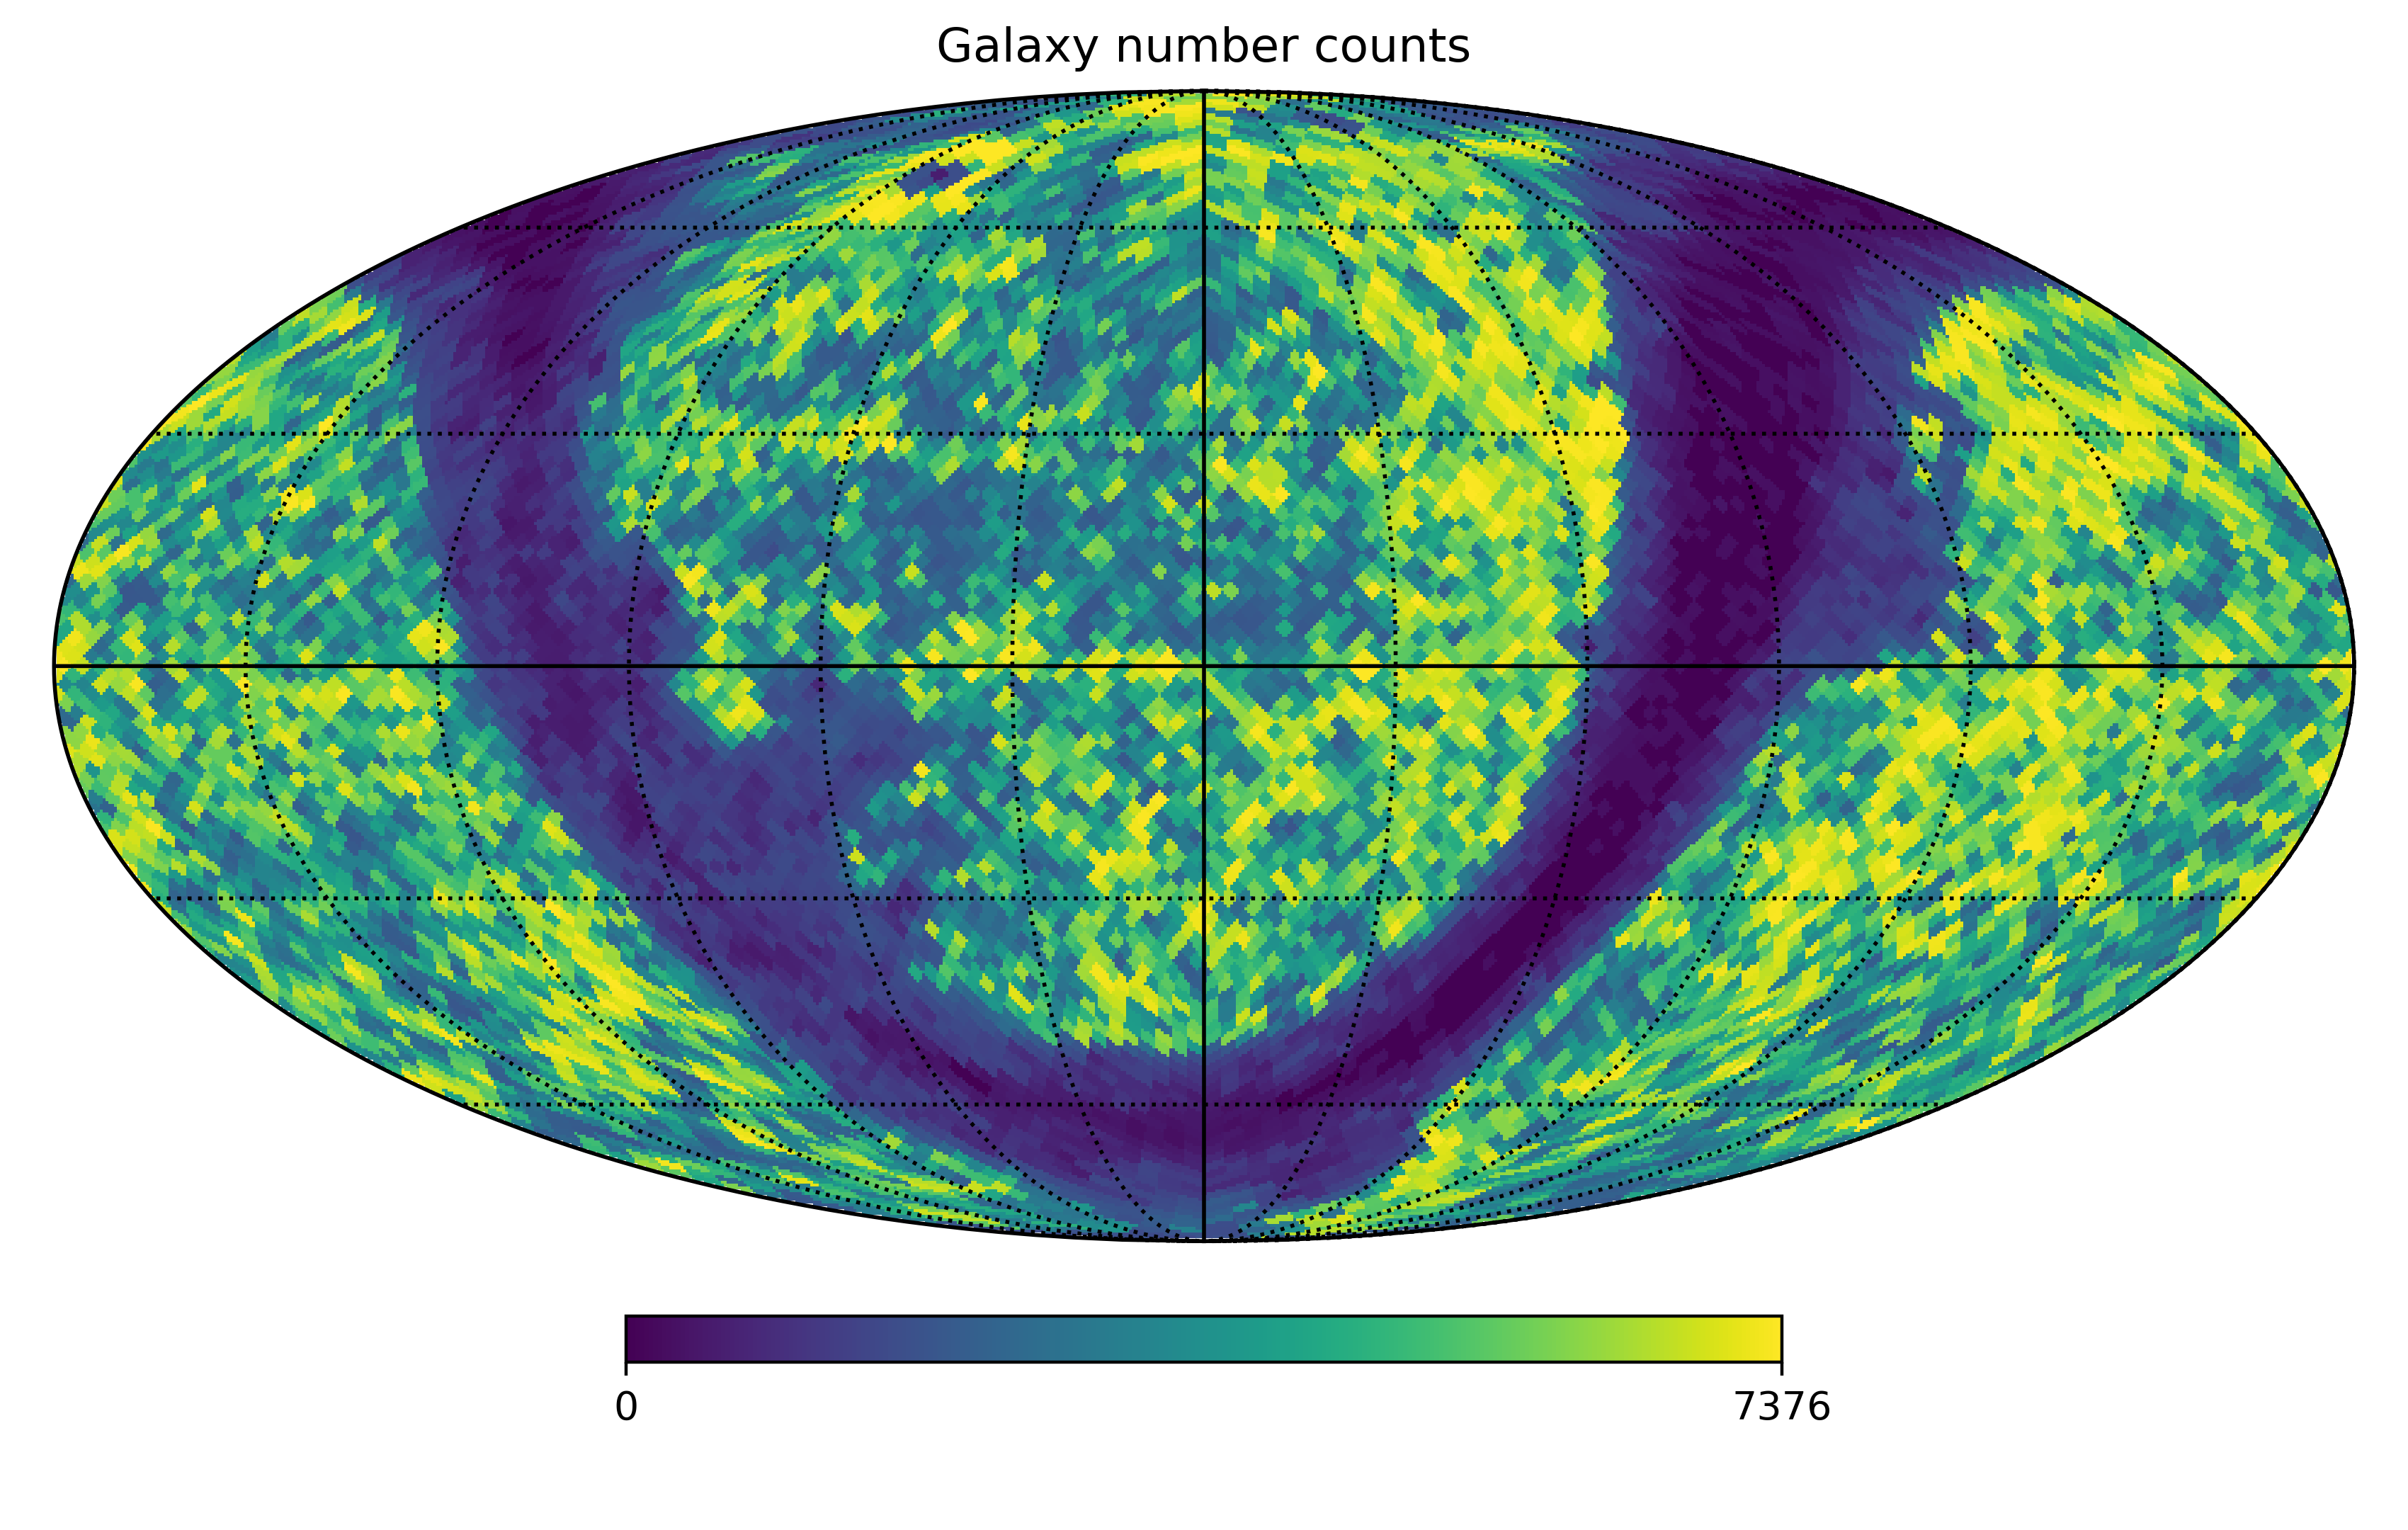
\includegraphics[width=\textwidth]{../src/figures/galaxy-map.png}
	\label{fig:galaxy-map}
\end{figure}

\begin{figure}[!ht]
	\caption{\textit{Left:} a histogram of the galaxy number count per redshift bin in the (whole-sky) catalog. \textit{Right:} the same histogram for all galaxies up to $z=1.5$.}
	\centering
	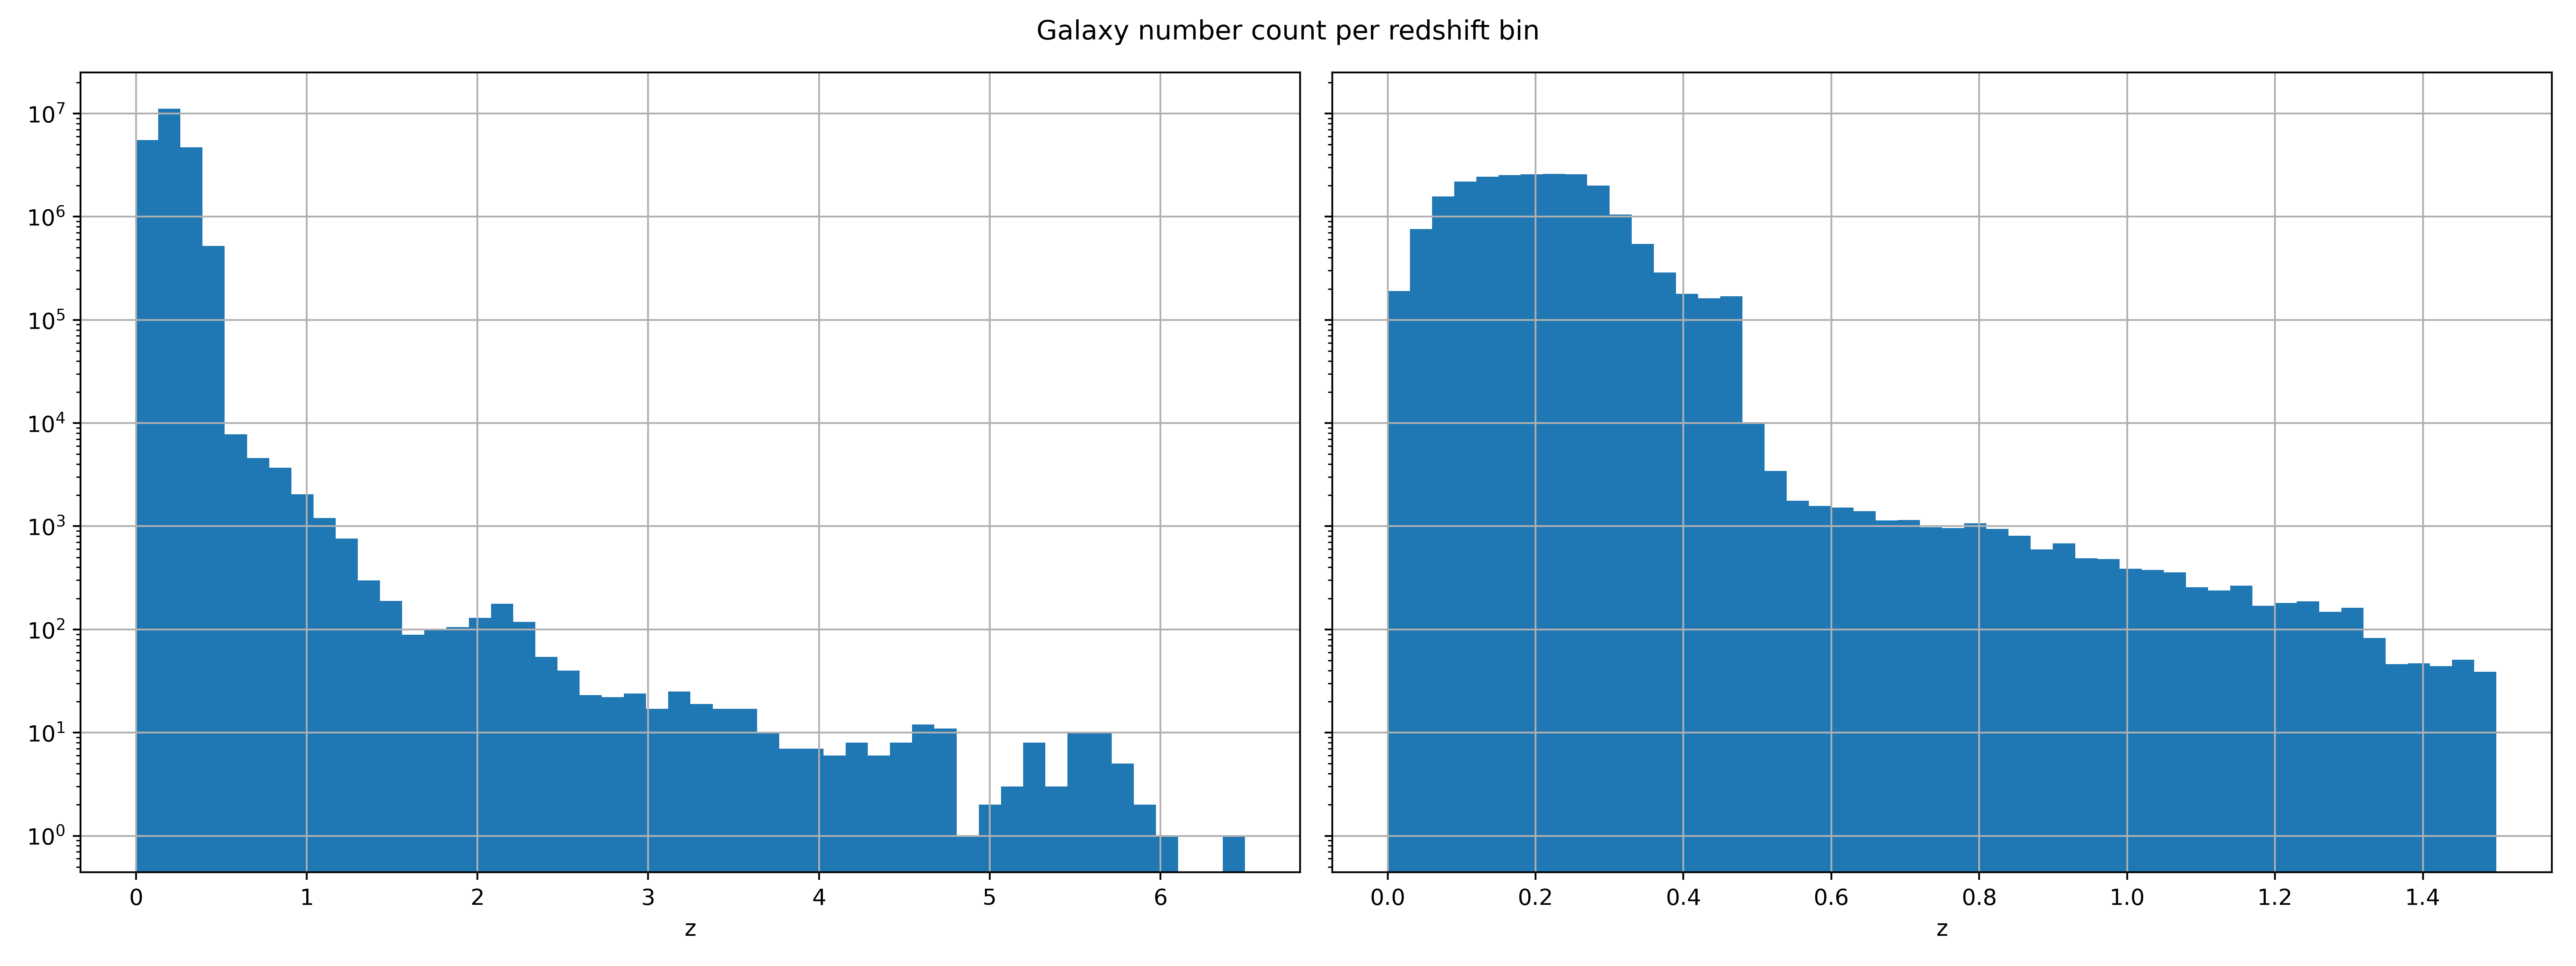
\includegraphics[width=\textwidth]{../src/figures/galaxy-redshift-distribution.png}
	\label{fig:galaxy-redshift-distribution}
\end{figure}

\subsection{The gravitational wave data}

The gravitational wave data is generated from the catalog directly:

\begin{enumerate}
	\item A direction $(\theta, \varphi)$ on the sky is picked, and all galaxies within an angular radius
	      $\alpha$ of it are selected as candidate hosts for the coalescences \footnote{The direction is
		      redrawn if there are less than $N_{\text{min}} \sim N_\text{GW}$ galaxies within it.}.
	\item A sample of $N_\text{gw}$ redshifts are drawn uniformly from said galaxies in the range $0 \leq z
		      \leq z_\text{max}$, where $z_\text{max}$ is a constant value fixed \textit{a priori}.
	\item The drawn redshifts are converted into \text{true} luminosity distances supposing a fiducial flat
	      $\Lambda$CDM cosmology with $\Omega_m = 0.3$ and $H_0 = 70 \, \rm{km} \, \rm{s}^{-1} \,
		      \rm{Mpc}^{-1}$. Each distance value is associated to a mock gravitational wave event.
	\item The \textit{measured} luminosity distances are drawn from their respective true values consistently
	      with the GW gaussian likelihood of Eq.~\eqref{eq:stat:gw-gaussian-likelihood}.

\end{enumerate}

To mitigate biases from the structure distribution in a particular direction, we sample mergers in
different directions and perform the inference on all of them.

Similar to HG23, we analyse two separate cases: the perfect-redshift limit and the full likelihood
from Eq.~\eqref{eq:stat:full-redshift-posterior}. We set $\sigma_L / d_L \in \{0.1, 0.2, 0.3\}$,
and we fix $z_\text{max} = 1.4$ and $d_L^{\rm{th}} = 1550 \,$Mpc. We choose a uniform prior $ H_0
	\in [20, 140] \, \rm{km} \, \rm{s}^{-1} \, \rm{Mpc}^{-1}$. Since we leave the remaining
cosmological parameters fixed, we implement a simple grid method to compute the marginalized
likelihood.

Our methodology is evidently a simple proof of concept of the galaxy catalog approach to dark siren
cosmography. Still, it is important to highlight the limitations to our method, as well as the
approximations that are made. Firstly, the simplified data-generating process: we are generating
mock events \textit{uniformly} from the available galaxies in the catalog. The resulting redshift
distribution of CBCs is inevitably inaccurate for two reasons: the galaxies may not equally be
likely to host these mergers; this may also be a function of their masses, luminosities,
metallicities, etc. Secondly, the galaxy distribution in the catalog does not reproduce the real
distribution due to the the latter's incompleteness. The selected redshifts will be artificially
small because of this. This should not spoil the analysis, so long as the mock events' generation
is consistent with the likelihood model. In particular, we expect that the posterior distribution
should peak around the fiducial value of $H_0$ used in the $z-d_L$ conversion. The galaxy
distribution in the catalog, however, is not expected to be reproduce this background cosmology.
Moreover, the (assumed true) redshifts of the coalescences are drawn from real measurements, and
therefore do not correspond to the true redshits of their corresponding hosts. This distinction
does not play a role when the spectroscopic$-z$ approximation is considered, namely the likelihood
in Eq.~\eqref{eq:stat:perfect-redshift-posterior}, although it becomes important for the broad case
where redshift uncertainty is incorporated into the analysis.

A number of approximations were also made in our likelihood model. The GW likelihood
$\given{\vec{d}}{\theta}$ does not, in general, follow a normal distribution. In real analyses,
while a similar ansatz can be used for the conditional probability of the distance to the event
given a sky direction~\cite{Singer_2016}, a more accurate procedure is to apply Bayes's theorem and
to discretely sample the posterior $\given{\theta}{\vec{d}}$ reconstructed in the single-event
parameter estimation with assumed prior $\pi (\theta)$~\cite{Mandel:2018mve}. Likewise, the
photo$-z$ PDF may be more complicated than Eq.~\eqref{eq:stat:photo-z-likelihood}, and can be
estimated with more sophisticated methods, such as neural
networks~\cite{Palmese_2023,alfradique2023dark}. Moreover, as already mentioned, a more realistic
computation of the selection effects involves injecting artificial signals and computing the number
of detections at the selected sensitivity. Finally, when using real GW data, the set of candidate
host galaxies should be extracted from the credible regions estimated from the events' skymaps -
for instance, with the \texttt{BAYESTAR} package~\cite{PhysRevD.93.024013}.

We have also explicitly ignored completeness corrections to the magnitude-limited galaxy catalog.
In our toy model, this is not as problematic since the CBCs are generated from the catalog itself.
In the general case, however, not accounting for the incompleteness will make the inference biased
as well as far less informative for events that occured at higher redshifts, which are commonplace
for BBHs. See Ref.~\onlinecite{dalang2023clustering} for a review of different completeness
corrections adopted in the literature.

The implementation is available in the Github link
\url{https://github.com/binado/standard-sirens/tree/main}. The goal of the repository is to make it
a playground for exploring different strategies for performing inference with standard sirens.

\rs{\subsection{Suggestions for development}}

\begin{itemize}
	\item Not all redshifts are equally probable, we expect a source distribution to follow somehow the
	      Madau-Dickinson one \cite{Madau:2014bja}: \be R(z)=\frac{dV}{dz}\psi(z) \ee where \be
	      \psi(z)=C_0\frac{(1+z)^\alpha}{\paq{1+\frac{1+z}B}^{\beta}}yr^{-1}Gpc^{-3} \ee

	      Is it possible to recover the valus of $\alpha,\beta, B$?

	\item Not all galaxies are equally probable, one can weigh them with the mass.

\end{itemize}

\rs{End of suggestions}

\section{Results and discussion}
\label{sec:results}

The results are presented in Figs.~\ref{fig:perfect-redshift-posterior} -
\ref{fig:full-inference-posterior}, for the spectroscopic-like and photometric-like redshift
uncertainties, respectively; Fig~\ref{fig:posterior-comparison} represents a side-by-side
comparison of both cases for different levels of luminosity distance uncertainty. As expected, a GW
likelihood with smaller uncertainty generates a more informative posterior. Nevertheless, since we
are dealing with simulated data, it is imporatant to keep in mind that the position and the height
of the posterior peaks fluctuate depending on the seed of the random generator used throughout the
code. Since each curve is generated from a set of independent mock events, it is thus not
meaningful to draw conclusions from their direct comparison out of single pipeline run. The
features in line-of-sight redshift distribution are imprints of the structure along that direction,
and the GW data, by construction, approximately reproduces them. To analyse the dependence of the
reconstructed posterior on the data in a quantitative manner, we run the inference pipeline
$N_\text{sim} = 100$ times, each with a different fiducial value of $H_0$ drawn uniformly from the
prior range $[20, 140] \, \rm{km} \, \rm{s}^{-1} \, \rm{Mpc}^{-1}$. We compute the minimal
symmetric $\alpha-$credible interval (CI) in which these fiducial values are located in the
corresponding posterior distributions. We then analyse the histogram distribution of $\alpha$. If
the inference is unbiased, we expect the fiducial values to lie within the symmetric CI with
percentile $\alpha$ a number $\alpha N_\text{sim}$ of times. This is an example of a p-p plot. This
procedure is computationally viable because our 1-dimensional posterior does not take longer than 1
minute to compute. In real analyses, however, where (multiple) cosmological parameters are jointly
estimated with, for instance, the black hole mass distribution, running several MCMC chains may be
intractable, or require a clever parallelization scheme. The p-p plots are represented in
Figs.~\ref{fig:pp-analysis-perfect-redshift}-\ref{fig:pp-analysis-full-inference}. We observe that
all curves approximately follow the straight 45$^{\circ}$ line which, as argued above, is the
expected behaviour for an unbiased inference. There are no significant deviations from it at any
interval.

\begin{figure}[!ht]
	\caption{The posterior probability distribution on $H_0$ for the inference under the perfect redshift measurement assumption,
		and different values of $C=\sigma_L / d_L$. The dotted black line represents the fiducial value used to generate the GW data.}
	\centering
	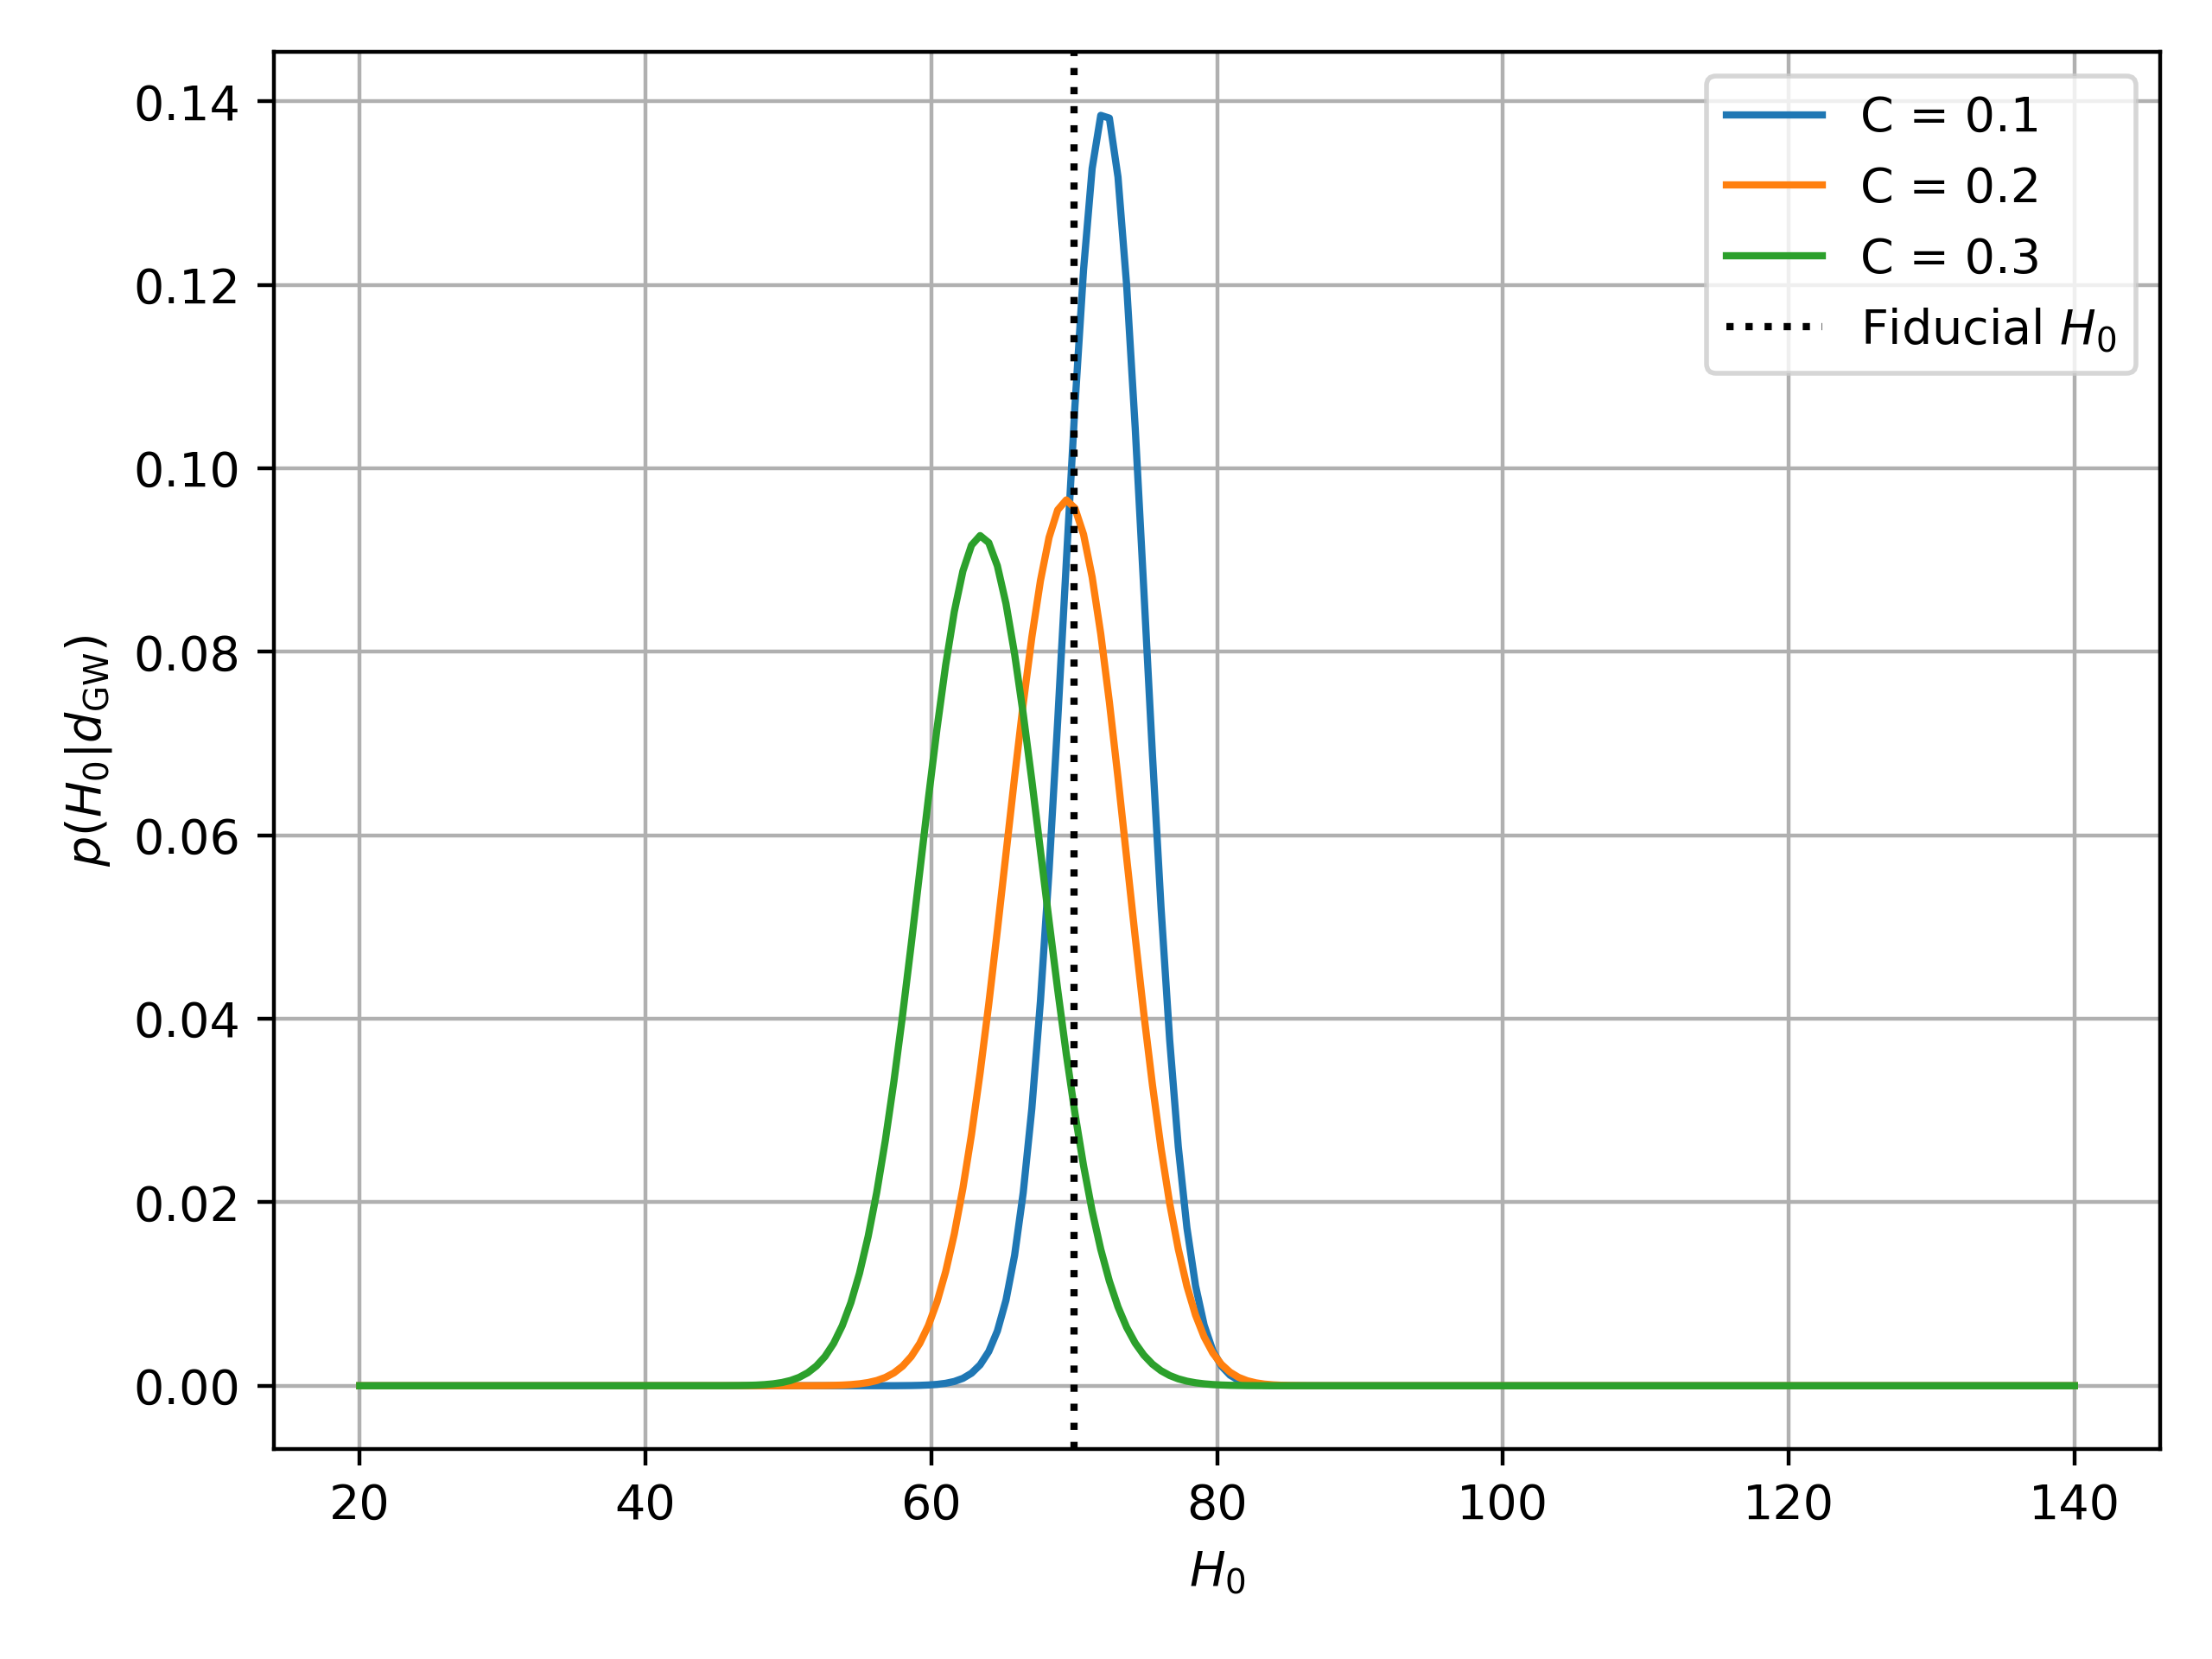
\includegraphics[width=0.8\textwidth]{../src/figures/perfect-redshift-posterior.png}
	\label{fig:perfect-redshift-posterior}
\end{figure}

\begin{figure}[!ht]
	\caption{The posterior probability distribution on $H_0$ for the inference under the normally distributed redshift measurement assumption,
		and different values of $C=\sigma_L / d_L$. The dotted black line represents the fiducial value used to generate the GW data.}
	\centering
	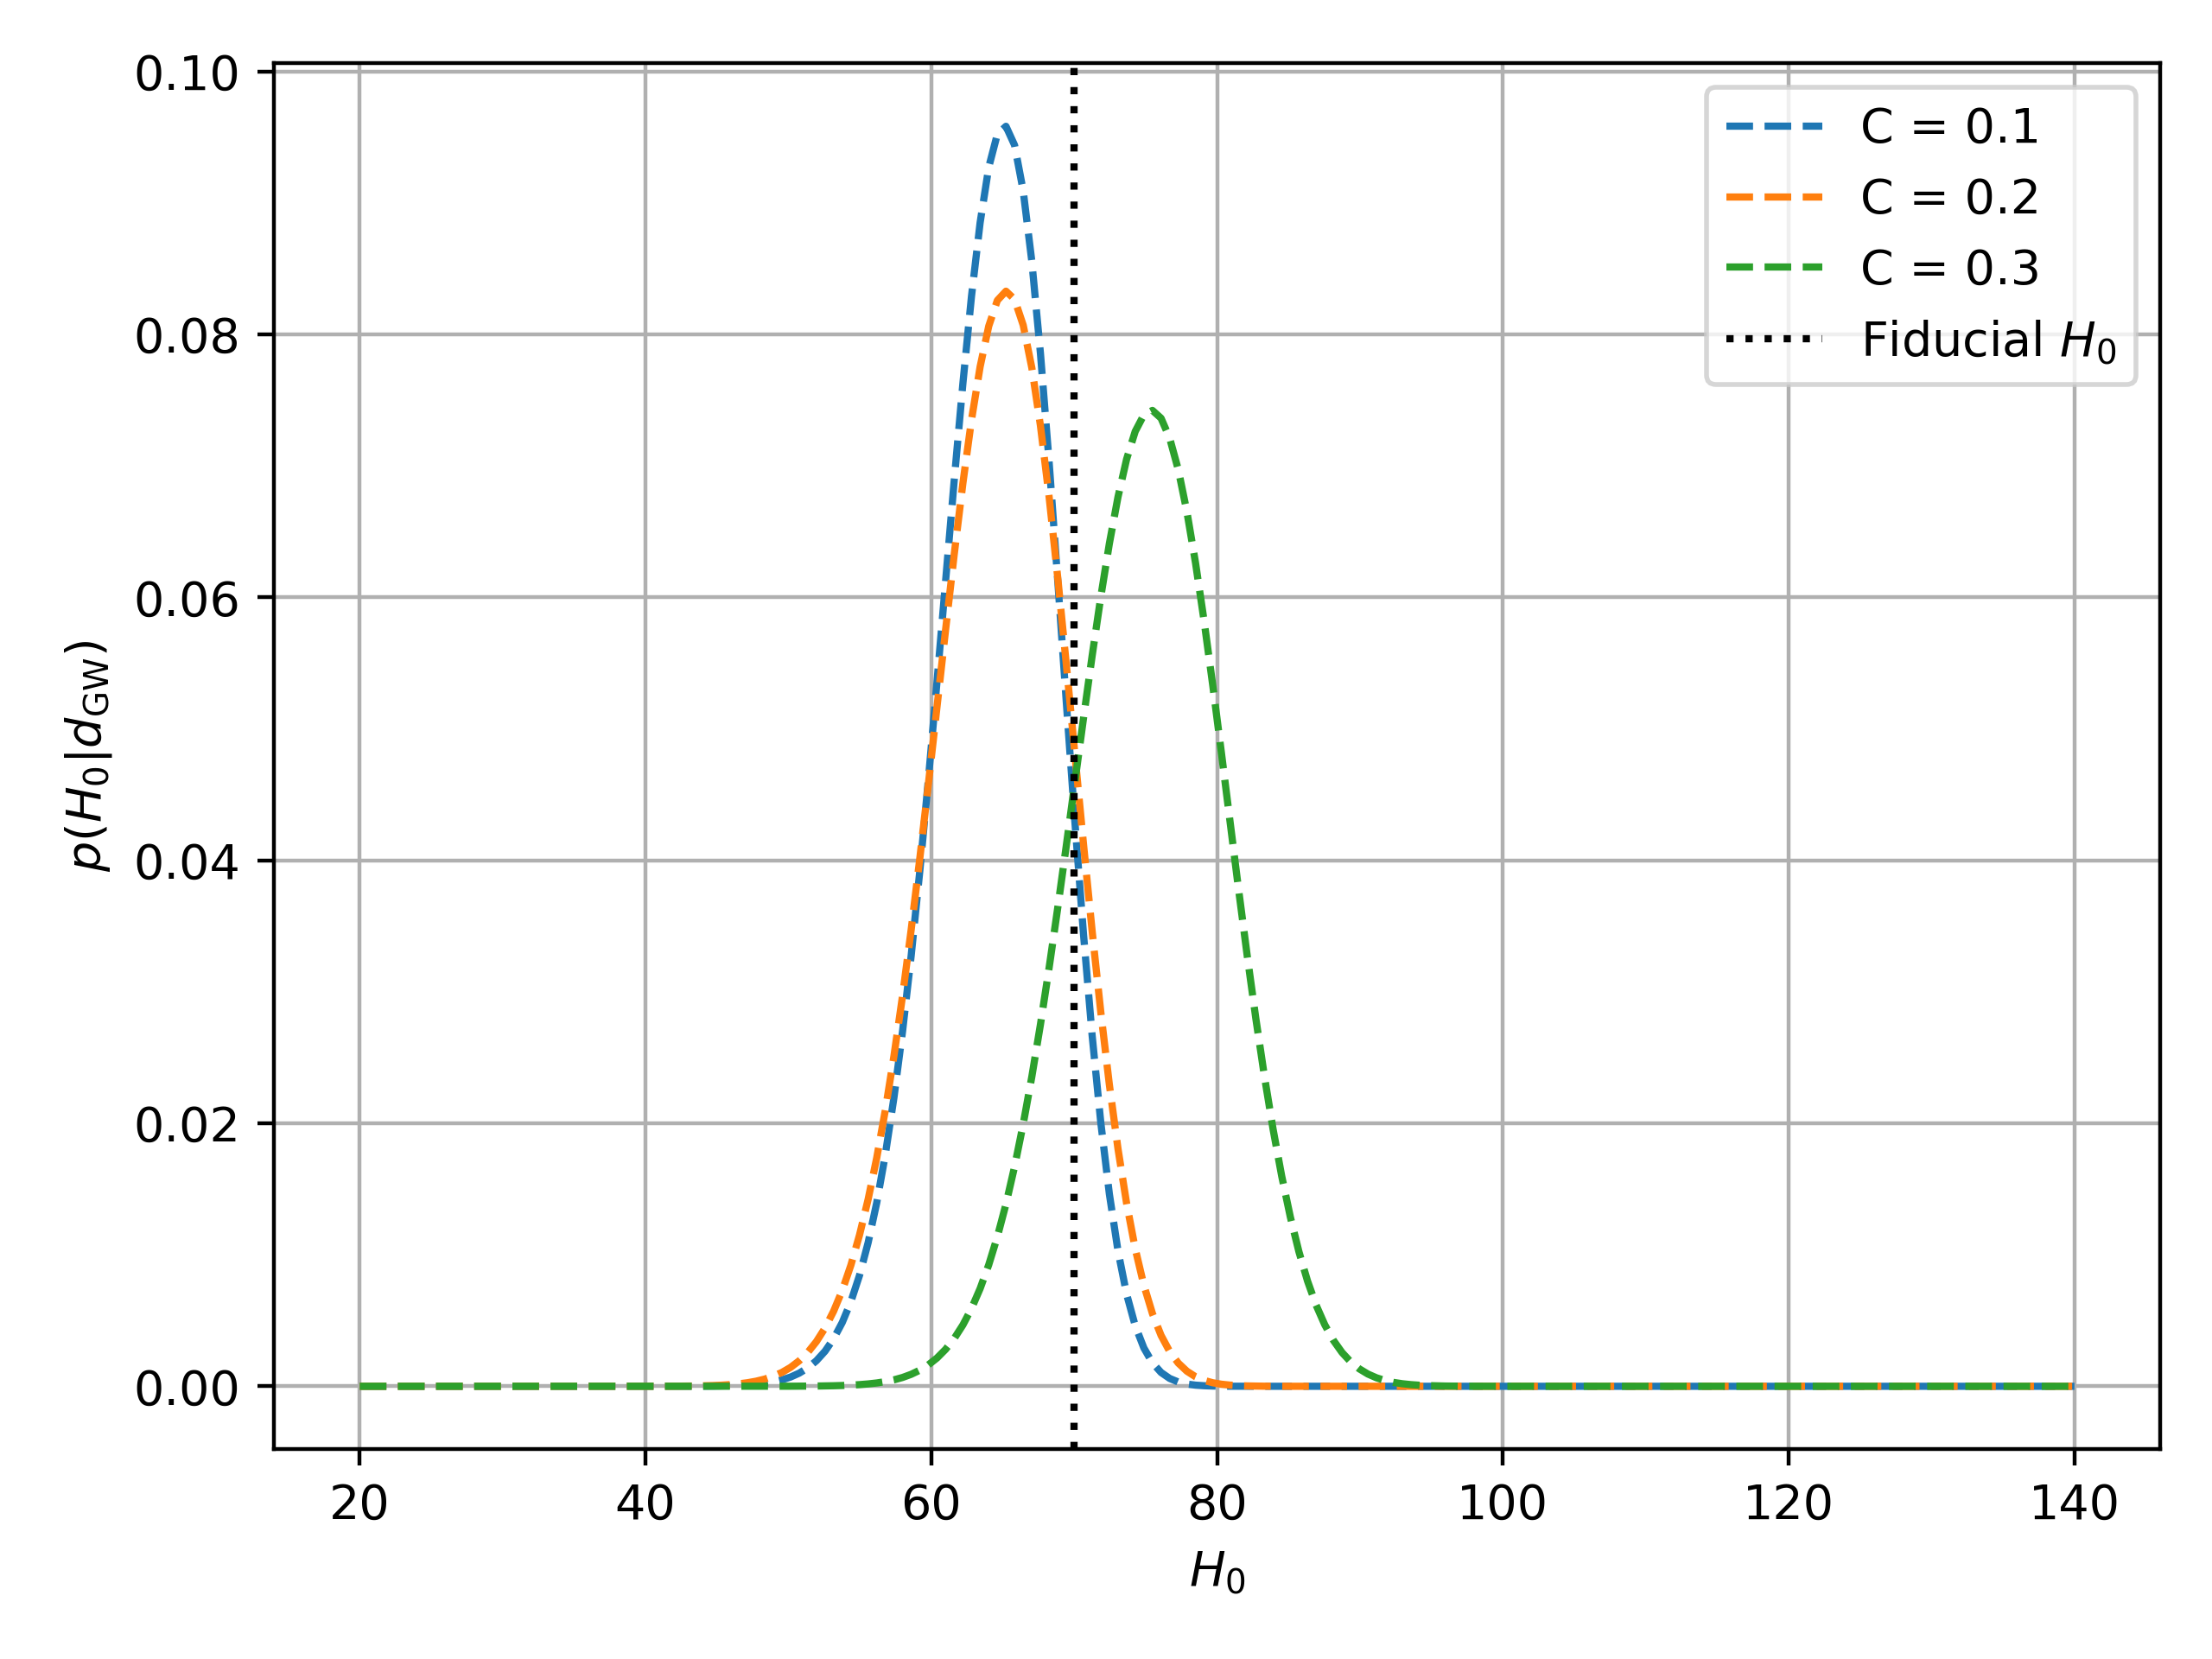
\includegraphics[width=0.8\textwidth]{../src/figures/full-inference-posterior.png}
	\label{fig:full-inference-posterior}
\end{figure}

\begin{figure}[!htpb]
	\caption{The posterior probability distribution on $H_0$ for the inference under both spec$-z$ and photo-$z$ cases,
		and for $C=0.1$ (top), $C=0.2$ (middle), and $C=0.3$ (bottom). The dotted black lines represent the fiducial value used to generate the GW data.}
	\centering
	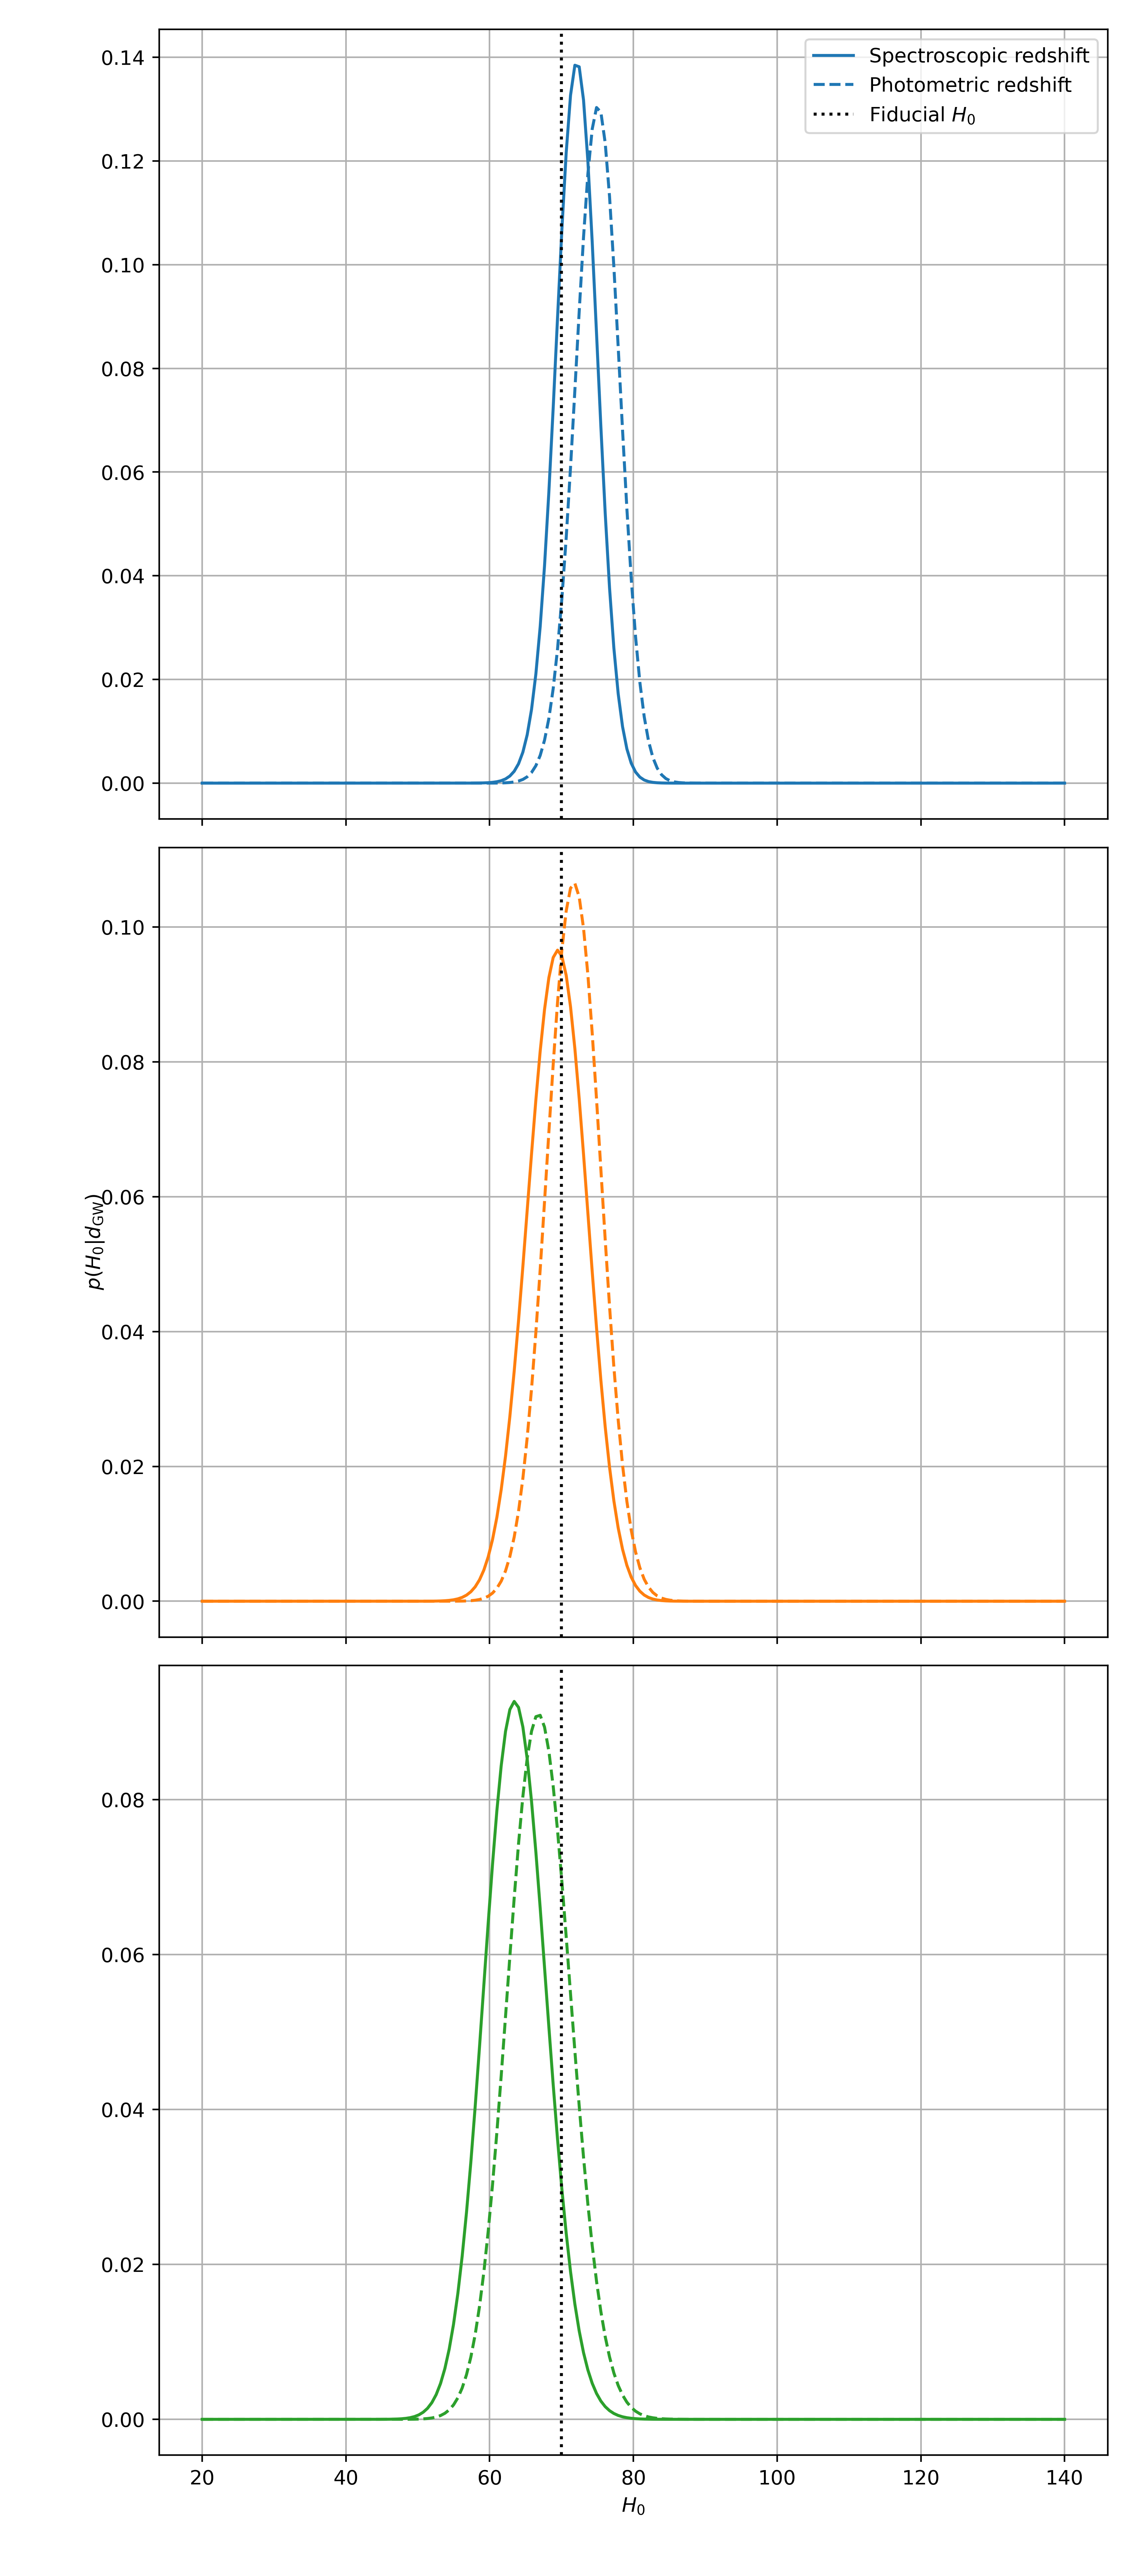
\includegraphics[height=0.9\textheight]{../src/figures/posterior-comparison.png}
	\label{fig:posterior-comparison}
\end{figure}

\newpage

\begin{figure}[!ht]
	\caption{p-p plot for the inference on perfect redshift measurement limit. The pipeline was run 100 times.
		The blue, orange and green curves correspond to $C=0.1 \, 0.2, \, 0.3$ respectively.
		The grey regions correspond to the $1\sigma$, $2\sigma$ and $3\sigma$ confidence levels.}
	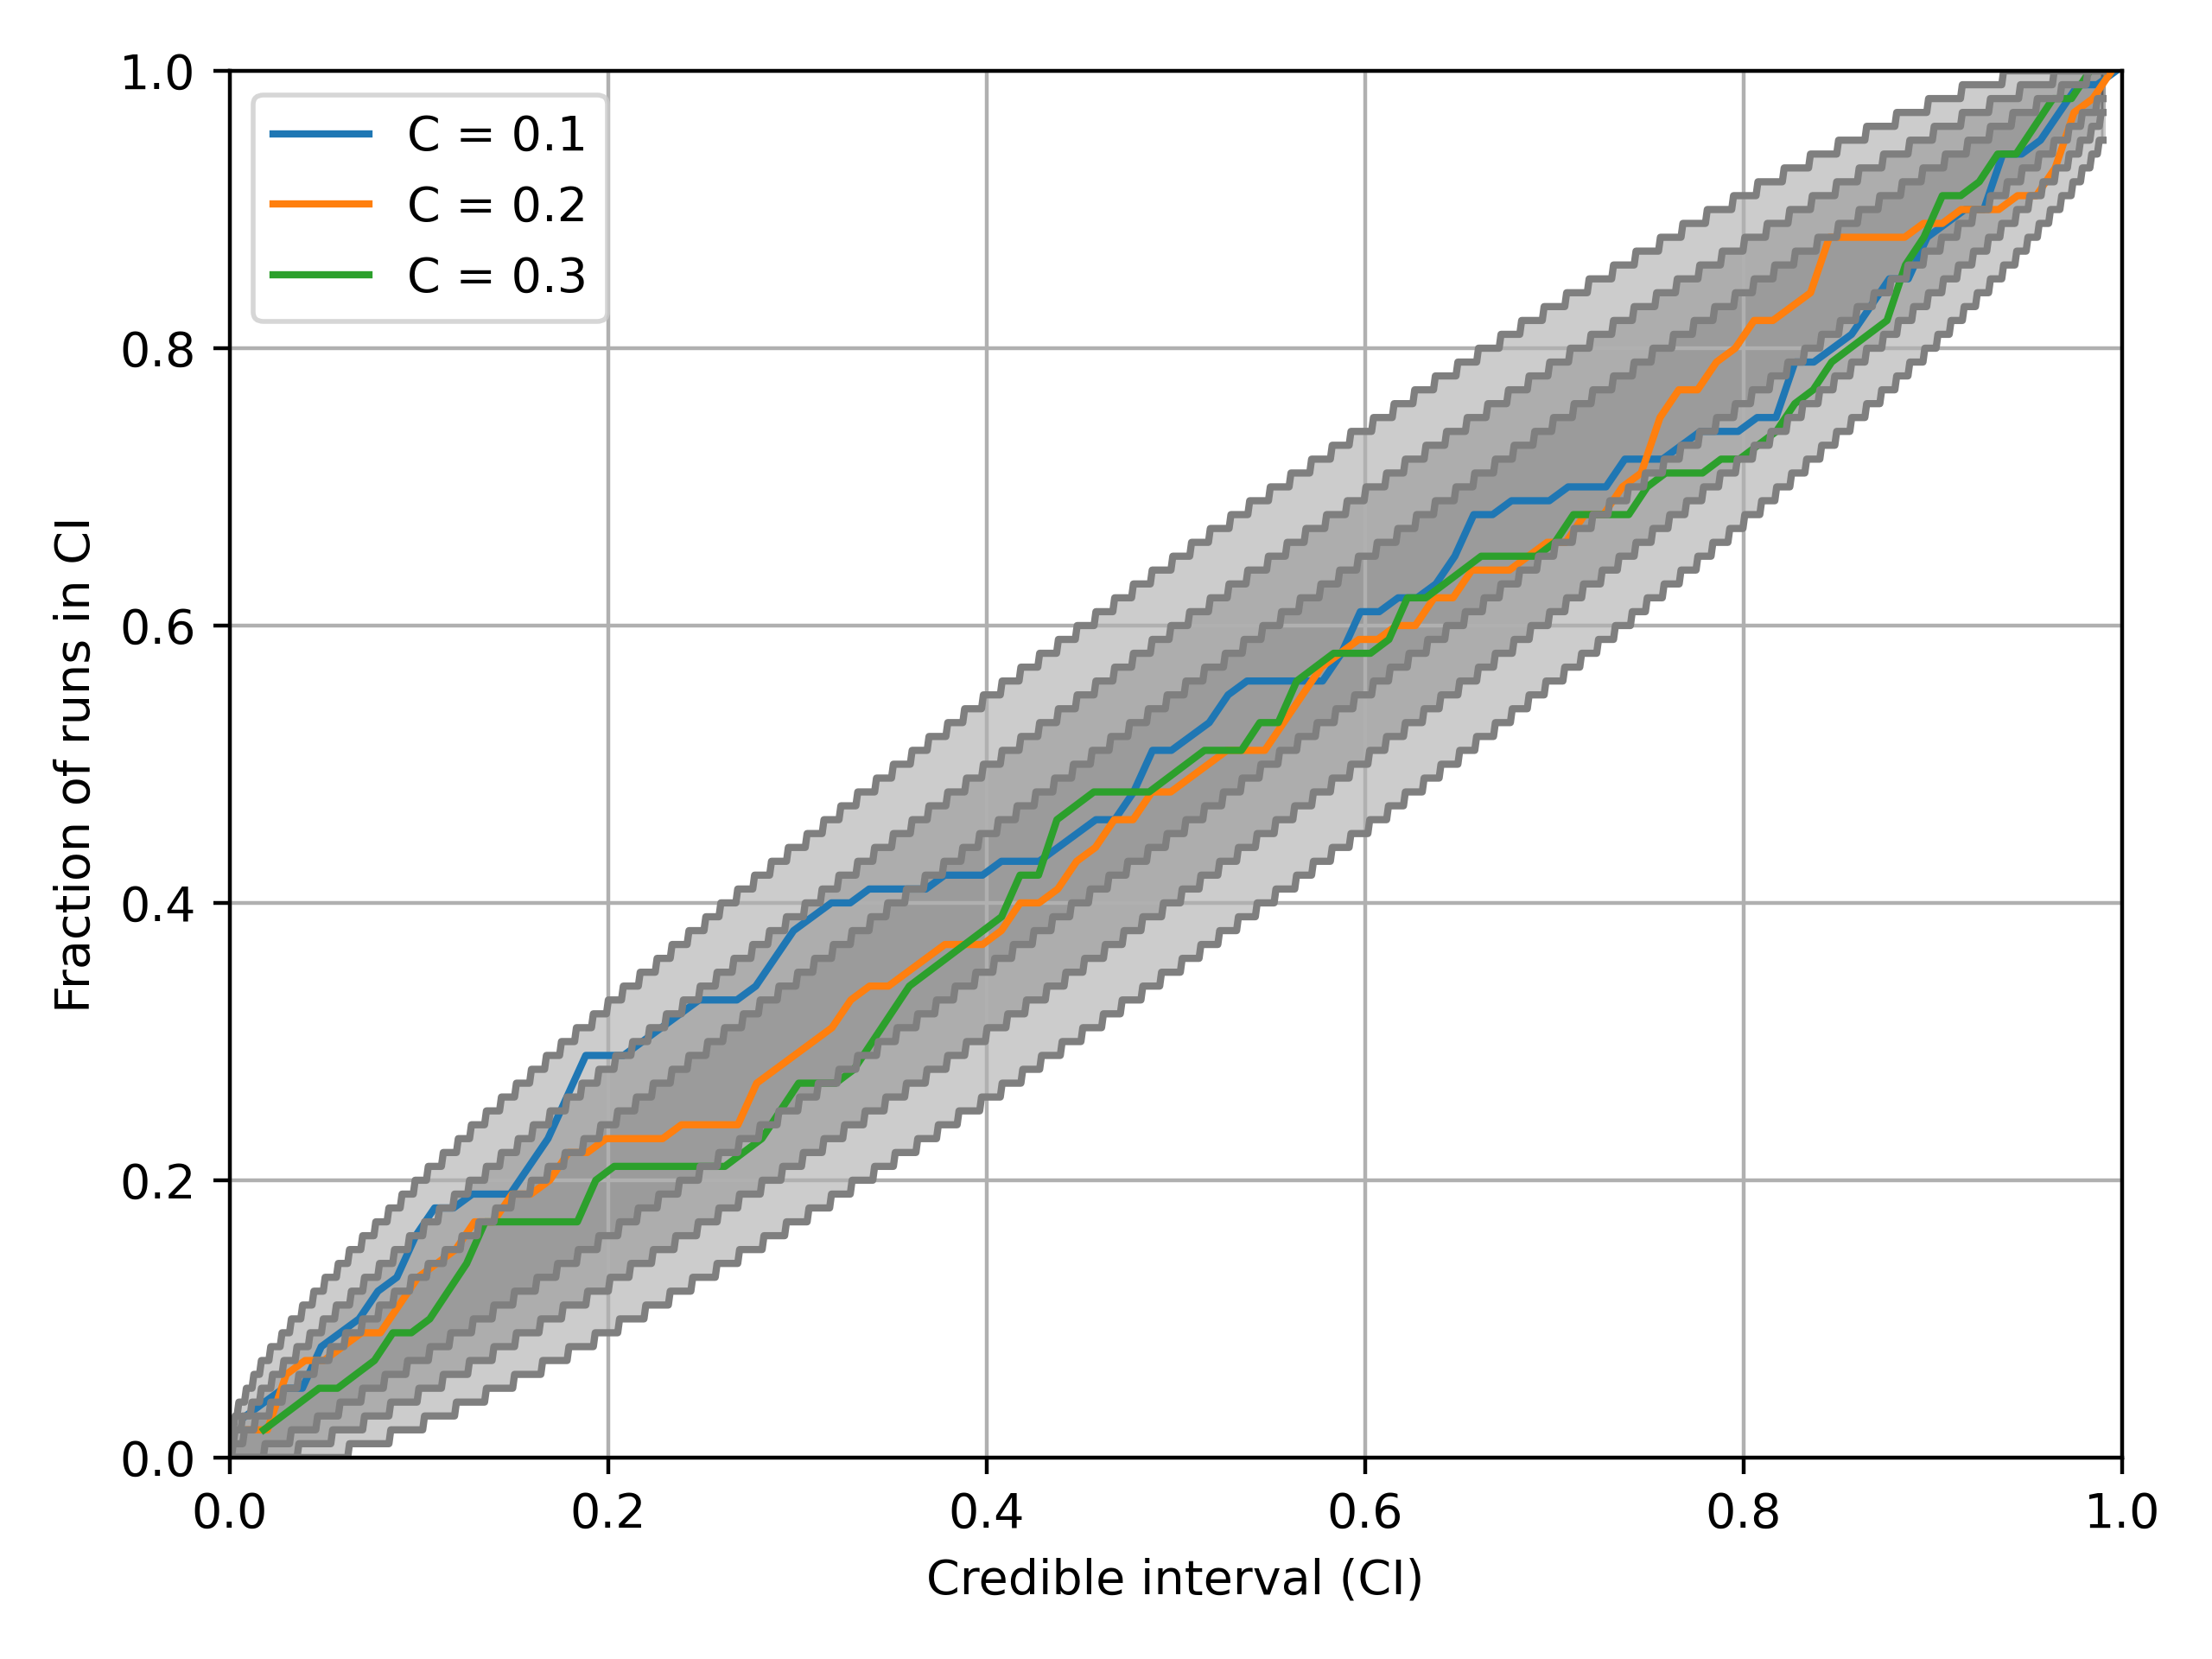
\includegraphics[width=0.8\textwidth]{../src/figures/pp-analysis-perfect-redshift.png}
	\label{fig:pp-analysis-perfect-redshift}
\end{figure}

\begin{figure}[!ht]
	\caption{p-p plot for the inference on perfect redshift measurement limit. The pipeline was run 100 times.
		The blue, orange and green curves correspond to $C=0.1 \, 0.2, \, 0.3$ respectively.
		The grey regions correspond to the $1\sigma$, $2\sigma$ and $3\sigma$ confidence levels.}
	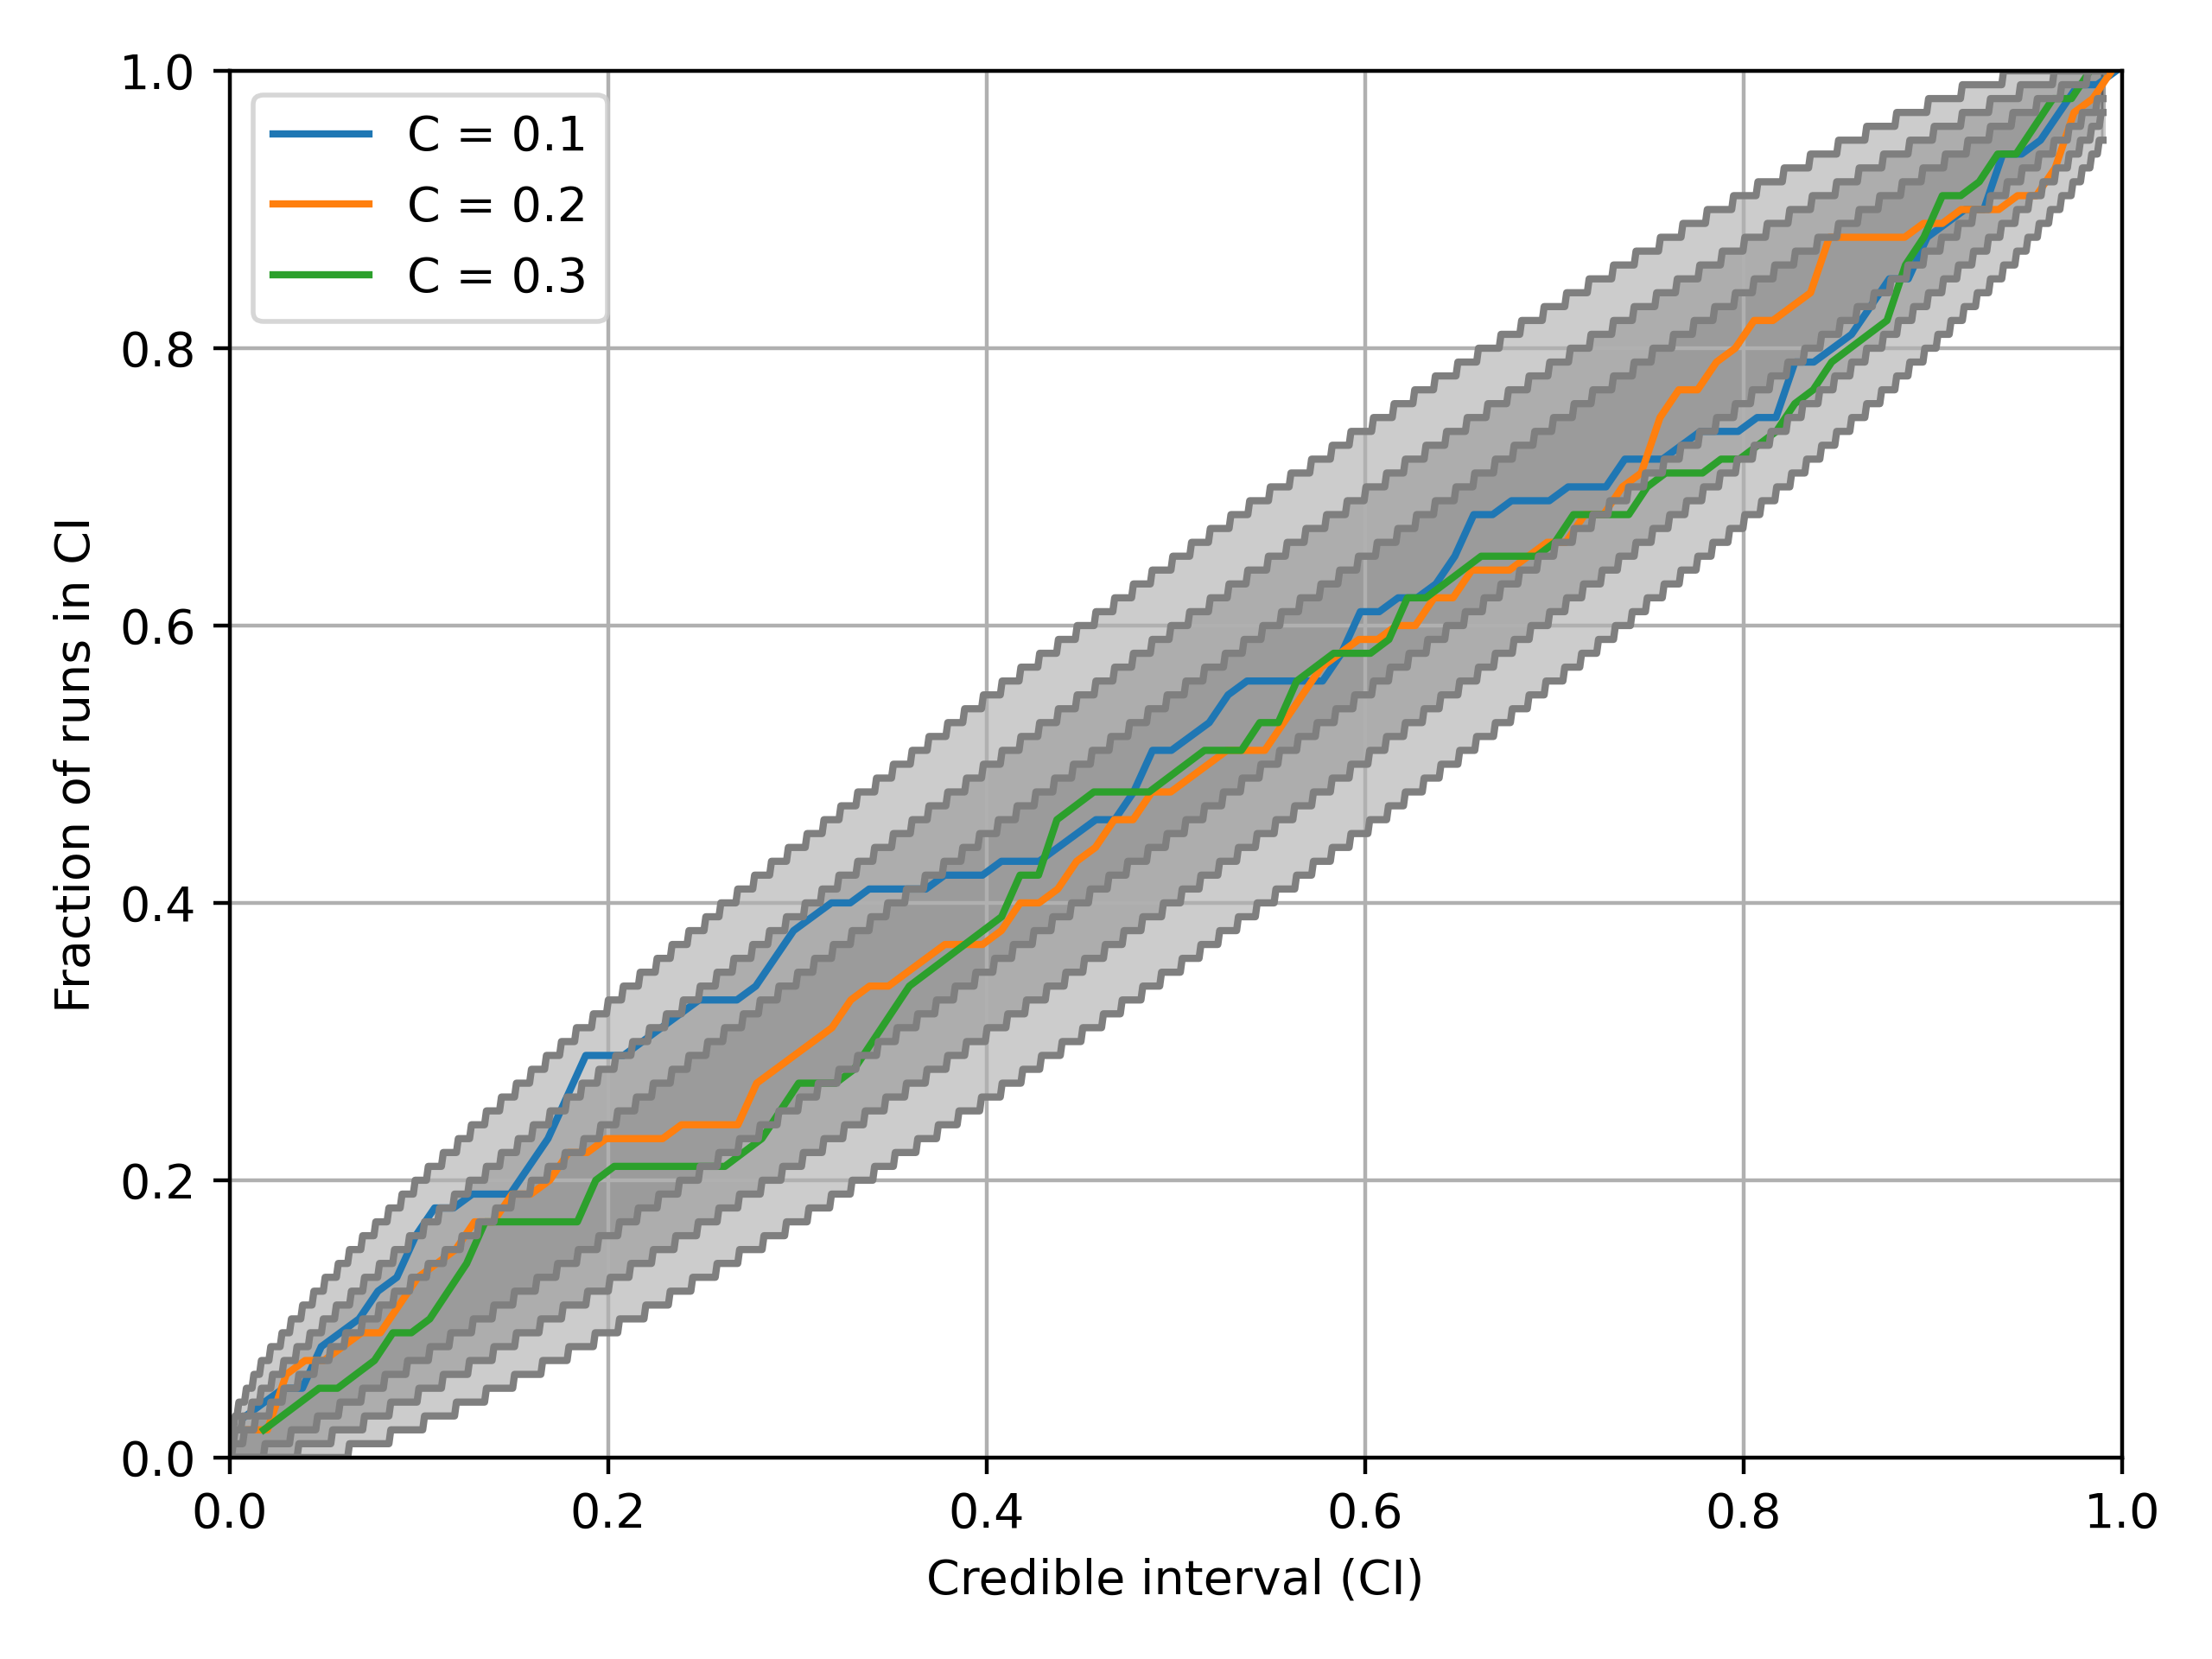
\includegraphics[width=0.8\textwidth]{../src/figures/pp-analysis-perfect-redshift.png}
	\label{fig:pp-analysis-full-inference}
\end{figure}

Finally, the analysis could take other directions as well. In HG23, the authors analysed limiting
cases in the object distributions, such as the few-galaxy, many-mergers configuration, where the
redshift of different CBC's may originate from the same host galaxy, in which case they are
correlated. We have also not explored the impact of the choice of fixed parameters, such as
$z_\text{max}$ or $d_L^{\text{th}}$, on the robustness of the results. Likewise, we could also
promote the remaining cosmological parameters to free hyperparameters of the model, and analyse the
impact on the constraining power on $H_0$.

\section{Conclusion}
\label{sec:conclusion}

This manuscript is intended as a pedagogical introduction to gravitational-wave standard sirens.
With more detections of mergers accumulated in the next LIGO-VIRGO-KAGRA runs, and especially with
the advent of third generation interferometer networks in the next decade, gravitational waves may
be a powerful and independent tool to measure the cosmic expansion history of the Universe.
Nevertheless, there are still challenges to deal with, which are mostly related to mitigating the
systematics in the process: the detector calibration uncertainty, the measurement uncertainty of
the source's luminosity distance, and so on. On the dark siren case, where no optical counterpart
is available, these systematic uncertainties are even more pronounced: while the informative power
of galaxy catalogs is significantly diminished at higher redshifts, using fixed BBH population
assumptions, which are more useful there, may dominate the outcome of the
inference~\cite{LIGOScientific:2021aug}. Therefore, while the standard-siren methodology is still
limited by statistical uncertainties, the multiple years of data collection process will be plenty
of time for scientists in the field to develop more sophisticated tools to model the systematics
into statistical uncertainties that can be marginalised over.

In the spirit of presenting pedagogical resources for a hands-on introduction to the field, we have
also presented a simple proof-of-concept implementation of an inference pipeline using simulated
dark sirens and the galaxy catalog method. Although our approach sligthly differs from
Ref.~\onlinecite{Gair_2023} in that the redshift data comes from a real catalog, \texttt{GLADE+},
we reach a similar conclusion, namely that that a data-generating process consistent with the
likelihood model assumptions led to an unbiased inference on the Hubble constant. A natural
extension of this work is to modify the implementation to work with real gravitational-wave data,
and to include other statistical methods studied in the literature, for instance incorporating
black hole population models.

\bibliography{refs}% Produces the bibliography via BibTeX.

\end{document}
%
% ****** End of file apssamp.tex ******
